% !TeX root = ./main.tex

\documentclass[12pt,twoside]{report}
\usepackage[english]{babel}
\usepackage[utf8]{inputenc}
\usepackage[a4paper,width=150mm,top=25mm,bottom=25mm,bindingoffset=6mm]{geometry}
\usepackage{csquotes}
\usepackage{graphicx}
\usepackage{amsmath}
\usepackage{enumitem}
\usepackage{changepage}
\graphicspath{ {./images/} }
\usepackage{caption}
\usepackage{subcaption}
\usepackage{ragged2e}
\usepackage{fancyhdr}
\usepackage[nottoc]{tocbibind}
\usepackage{xurl}
\usepackage{wrapfig}
\usepackage{float}

\usepackage{listings}
\usepackage[nottoc]{tocbibind}
\usepackage[chapter]{minted}
\usemintedstyle{vs}

\lstset{
    % float=H
    breaklines=true,
}


\usepackage{chngcntr}
\AtBeginDocument{\counterwithin{lstlisting}{section}}


\pagestyle{fancy}
\fancyhead{}
\fancyhead[RO,LE]{Music and Feelings:  A Deep Learning Approach to Emotional Composition}
\fancyfoot{}
\fancyfoot[LE,RO]{\thepage}
\fancyfoot[LO,CE]{Chapter \thechapter}
\fancyfoot[CO,RE]{Naiman Alexandru Nicolae}
\renewcommand{\headrulewidth}{0.4pt}
\renewcommand{\footrulewidth}{0.4pt}
\setlength{\parindent}{0pt}
\setlength{\parskip}{1em}
\usepackage[parfill]{parskip}
\newcommand{\code}[1]{\texttt{#1}}

% \renewcommand{\baselinestretch}{1.5}
\usepackage{setspace}
\setstretch{1.25}


\title{Thesis Title}
\author{Author Name}
\date{Day Month Year}

\begin{document}
\begin{titlepage}
    \begin{center}

        \large
        {BABES-BOLYAI UNIVERSITY CLUJ-NAPOCA\\
            \vspace{0.5cm}
            FACULTY OF MATHEMATICS AND COMPUTER SCIENCE\\
            \vspace{0.5cm}
            SPECIALIZATION COMPUTER SCIENCE}

        \vfill


        \Large
        \textbf{DIPLOMA THESIS}

        \vspace{0.5cm}
        \Large
        \textbf{Music and Feelings: A deep learning approach to emotional composition}

        \vfill

        % Supervisor part
        \begin{justify}
            \textbf{Supervisor:\\}
            Darabant Sergiu Adrian
        \end{justify}

        \vspace{0.8cm}

        % Author part
        \begin{flushright}
            \textbf{Author:\\}
            Naiman Alexandru Nicolae
        \end{flushright}
        % \includegraphics[width=0.4\textwidth]{university}

        \vspace{2cm}


        Cluj-Napoca\\
        2020

    \end{center}
\end{titlepage}
\begin{titlepage}
    \begin{center}

        \large
        \textbf{UNIVERSITATEA BABEŞ-BOLYAI CLUJ-NAPOCA\\
            \vspace{0.5cm}
            FACULTATEA DE MATEMATICǍ ŞI INFORMATICǍ \\
            \vspace{0.5cm}
            SPECIALIZAREA INFORMATICǍ ÎN LIMBA ENGLEZǍ}

        \vfill


        \Large
        \textbf{LUCRARE DE LICENŢĂ}

        \vspace{0.5cm}
        \Large
        \textbf{Muzică și sentimente: O abordare fondată pe învatare profundă a compoziției muzicii pe baza emoțiilor}

        \vfill

        % Supervisor part
        \begin{justify}
            \textbf{Conducător ştiinţific:\\}
            Conf. Univ. Dr. DARABANT Sergiu Adrian
        \end{justify}

        \vspace{0.8cm}

        % Author part
        \begin{flushright}
            \textbf{Absolvent:\\}
            Naiman Alexandru Nicolae
        \end{flushright}
        % \includegraphics[width=0.4\textwidth]{university}

        \vspace{2cm}


        \textbf{2020}

    \end{center}
\end{titlepage}

\thispagestyle{plain}
\begin{center}
    \Large
    \textbf{Abstract}

    \vspace{0.4cm}
    % \large
    % Thesis Subtitle

    % \vspace{0.4cm}
    % \textbf{Author Name}

    % \vspace{0.9cm}
    % \textbf{Abstract}
\end{center}
Year after year, the music industry sets new records on their revenue,
earning billions of dollars through different mediums,
from LP records to  CDs, and with the rise of the Internet,
through streaming platforms.
This growth can be associated with the ease of producing
and releasing new songs, processes that have been facilitated
through different tools such as Digital Audio Workstations
and Virtual Studio Technology plugins. Even with all these advancements,
the approach one has when composing did not change in the last hundreds of
years: composing based on inspiration with a combination of
trial and error corrected by music theory.

This thesis introduces a tool designed for easing music composition,
flattening the steep learning curve of music theory,
by helping to compose songs based on feelings.
The main goal of the application is providing the user with a way of
generating songs based on some emotion given data.
The user provides the input emotion values,
and the software should respond with a composed song in which one can
recognise the given emotion.

The application consists of two parts:
the frontend web application with which the user interacts,
and the backend on which our machine learning model is running.
For the emotion data, the valence-arousal classification was used,
which specifies that any feeling can be expressed through the two aforementioned
values. For the composing algorithm, the autoencoders were used
for their capabilities of learning the internal structure of the
data, then used it for generating new songs based on new input.

This work is the result of my activity.
I have neither given nor received unauthorized assistance on this work.


% \chapter*{Dedication}
% To mum and dad

% \chapter*{Declaration}
% I declare that..

% \chapter*{Acknowledgements}
% I want to thank...

\tableofcontents

\listoffigures

\renewcommand\listoflistingscaption{List of Source Codes}
\listoflistings
\addcontentsline{toc}{chapter}{List of Source Codes}

% \listoftables



% \begin{justify}

\chapter{Introduction}
“Music is a moral law. It gives a soul to the Universe, wings to the mind, flight to the imagination, a charm to sadness, gaiety and life to everything.
It is the essence of order, and leads to all that is good and just and beautiful.” \cite{quotationDictionary}\\
\vspace{0.5cm}
Music is a collection of coordinated sounds \cite{whatIsMusic} whose medium is sound,
being one of the first ways of expressing the human had ever had.
From childhood to late adult life, we find ourselves listening to music, according to our feelings:
from babies’ lullabies to calm our little kids, to the most hyper energetic metal or drum and bass to keep us awake when learning for the finals.\\
\vspace{0.5cm}
The art of composing music is not one that any beginner can master due to the fact that
music theory has a very steep learning curve.
You can still compose music, without knowing anything about theory,
but it will be very hard to know how to really express your thoughts since the notes do not have any meaning to you other than their sound.
When you start learning, you will find out about scales, modes, chords progression and how they clearly relate to some feelings.\\
\vspace{0.5cm}
I want to encourage and help all people that have difficulties composing music with the help of machine learning.
I want to create an application that can compose, enhance or continue a piece of music based on some emotions that the user can provide.
The music should have a structure and the app will generate a MIDI file containing a song with the given characteristics.


\chapter{Machine Learning and Autoencoders}
This chapter contains theoretical information about the paper's domain, deep learning,
and the principal model used, autoencoders.
Of course, before starting looking in its domain,
we should start with the basics, namely, machine learning.
\section{What is Machine Learning?}

Machine learning is one of many subfields of artificial intelligence,
the science of getting the computer to learn from experience
without being explicitly programmed to do so,
improving their ability to think, plan, decide, etc. \cite{whatIsML}.\par
Algorithms in this area are different in their approach, the type of data they input and output,
and the type of problem they are learning to
solve, but, despite all differences, they are based on the same idea that there are some
generic algorithms that can discover patterns,
without having to write code; instead, they build their own logic on the data fed to them.
% \vspace{0.5cm}

% @HERE
\section{Machine Learning Styles}
When studying machine learning, one can identify a plethora of algorithms,
each unique in its approach and purpose, but all of them can be classified
based on the learning style. Therefore, there can be grouped into four main categories:
\begin{itemize}
    \item \textbf{Supervised Learning}
    \item \textbf{Unsupervised Learning}
    \item \textbf{Semi-supervised Learning}
    \item \textbf{Reinforcement Learning}
\end{itemize}
\vspace{0.5cm}

% @HERE
\subsection{Supervised Learning}
In supervised learning, given a set of example input-output pairs,
the job of the algorithms is to approximate a function that maps from input to output \cite{amai}.
It is called supervised learning because human experts act as the teacher,
where they serve the computer with training data containing the input and
also provide the correct output, from which the computer should be able to observe patterns.
As depicted in Figure\emph{~\ref{fig:supervised}},
the algorithm should be able to predict the output when given new inputs,
based on the function that it approximates \cite{typesMLMedium}.

\begin{figure}[h]
    \centering
    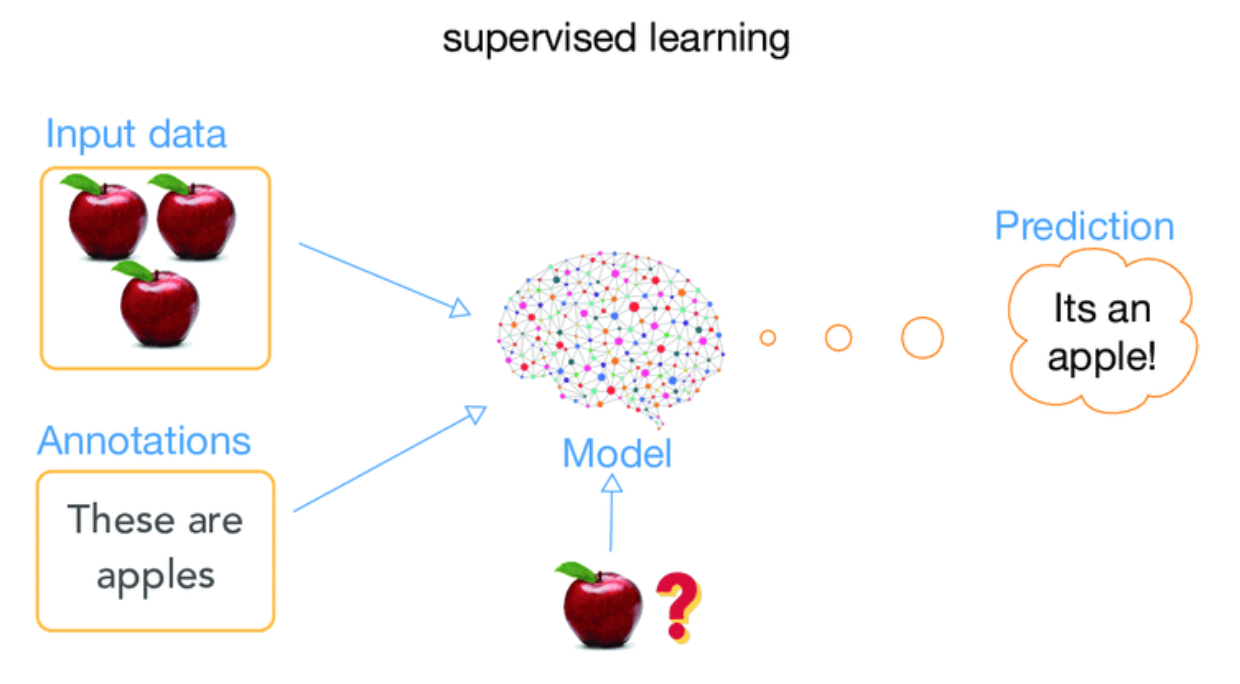
\includegraphics[width=1\textwidth]{supervised_learning}
    \caption{\emph{Supervised algorithm predicting new output data given new input  \cite{typesML}}}
    \label{fig:supervised}
\end{figure}

Furthermore, supervised machine learning algorithms can also
be grouped based on the type of problem they intend to solve.
Having said that, there are classification and regression algorithms.

% @HERE Classification
Classification algorithms solve problems in which the input data has
been labelled in different classes or categories,
meaning that the goal is to predict discrete values
such as $\{0, 1\}$, $\{2, 4, 6, 8\dots\}$, $\{cat, dog\}$, $\{spam, normal\}$, etc \cite{typesMLMedium}.

% @HERE Regression
Regression algorithms, on the other hand, solve problems in which the output variable
is a real value, meaning that the goal is to predict continuous values based on the
input data, such as predicting house prices based on their size and location \cite{typesMLMedium}.

\begin{figure}[h]
    \centering
    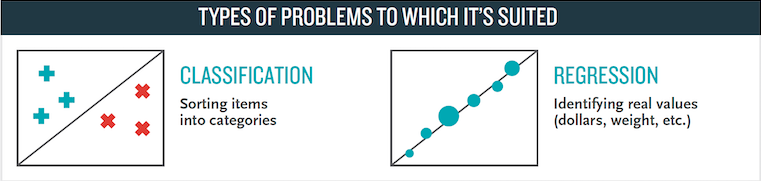
\includegraphics[width=0.8\textwidth]{regression_classification}
    \caption{\emph{Classification(left) and Regression(right) visualization  \cite{bigDataR}}}
    \label{fig:regression_classification}
\end{figure}


\subsection{Unsupervised Learning}
In unsupervised learning, the job of the algorithms is to observe patterns in
the structure of the given data even though no explicit feedback is supplied \cite{amai}.
There is no human factor implied in the learning process,
hence the name of unsupervised learning.
As shown in Figure\emph{~\ref{fig:unsupervised}}, they should be able to identify the underlying
structure in the given data, to better understand it \cite{bigDataR}.

\begin{figure}[h]
    \centering
    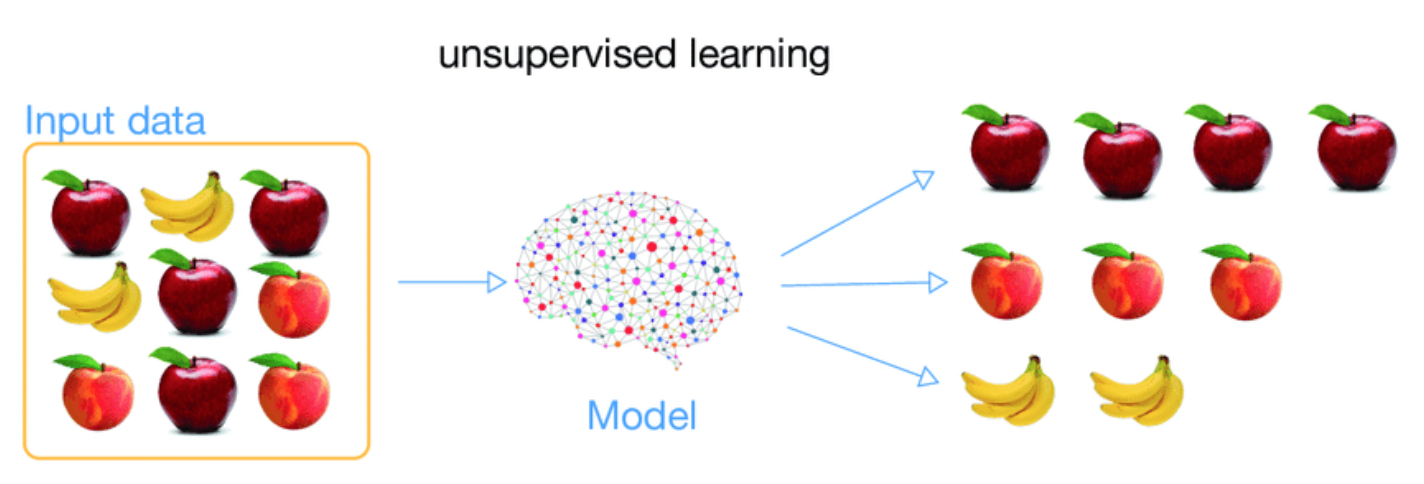
\includegraphics[width=1\textwidth]{unsupervised_learning}
    \caption{\emph{Unsupervised algorithm grouping data by their observed features \cite{typesML}}}
    \label{fig:unsupervised}
\end{figure}

The same as supervised learning, unsupervised algorithms can also be grouped
based on the type of problem they intend to solve. Provided that,
there are clustering and low-dimensional embedding algorithms \cite{amai}.

%  @HERE clustering
Clustering algorithms try to solve problems by grouping the input data
into different segments based on similarities learned,
such as grouping customers by purchasing behaviour \cite{brownlee2016master}.


% @HERE dimensionality reduction
Low-dimensional embedding, also called dimensionality reduction,
is a technique in which complex data, that is difficult to describe
(data that needs more than two or three dimensions to represent)
is reduced to a lower number of dimensions,
wherein the machine learning algorithms can help
since they can learn the internal structure inside our data, furthermore,
transcribing it to an easier way of interpreting it \cite{amai}.


\subsection{Semi-supervised Learning}
Semi-supervised learning algorithms lie between the aforementioned categories.
They intend to solve problems where you have a large amount of data but only some labelled.
A lot of machine learning problems are using this technique for the reason that
labelled data can be expensive or time-consuming to obtain,
in contrast to unlabelled data that is much easier to acquire \cite{brownlee2016master}.

As shown in Figure\emph{~\ref{fig:semi_supervised_learning}}, one can use an initial classifier on the labelled data,
classify based on the features learned previously, the unlabelled data,
retrain the classifier with the whole dataset,
then use it to predict new outputs given new input data, ideally obtaining a better model \cite{lotte2015}

\begin{figure}[h]
    \centering
    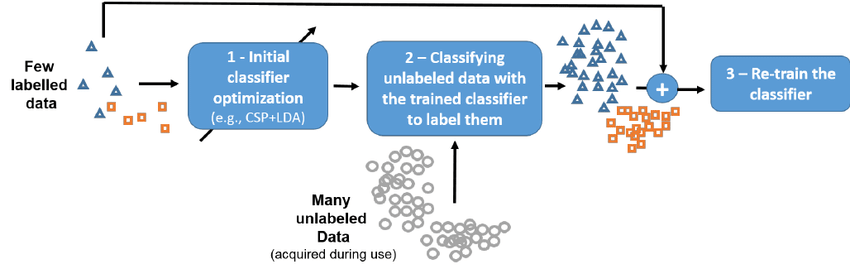
\includegraphics[width=1\textwidth]{semi_supervised_learning}
    \caption{\emph{Semi-supervised approach on data classification \cite{lotte2015}}}
    \label{fig:semi_supervised_learning}
\end{figure}

\subsection{Reinforcement Learning}
Reinforcement learning algorithms are based on a system of type reward-punishment,
where the job of the algorithm is to iteratively interact with its environment,
making actions in such a manner that will maximize the rewards or minimize the punishments.
To put it another way, in reinforcement learning,
the software learns from its past experiences allowing it to develop an optimal
behaviour within a specific setting, where it aims to increase its performance \cite{typesMLMedium}.

\begin{figure}[h]
    \centering
    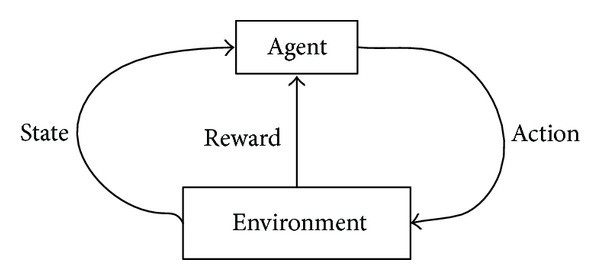
\includegraphics[width=1\textwidth]{reinforcement_learning}
    \caption{\emph{Scheme of how reinforcement algorithms work \cite{typesMLMedium}}}
    \label{fig:reinforcement_learning}
\end{figure}

Figure\emph{~\ref{fig:reinforcement_learning}} is a visual representation of how reinforcement learning works. The algorithm
(called the "agent" in the picture), takes action in the environment,
which will possibly trigger a reward. After that, the state is updated,
and when deciding its next action, it will take into account its last state and the
result of the previous action.

\section{ANNs and how they work}
One of the main types of machine learning algorithms that are vastly used is
artificial neural networks or ANNs.
They are structured as weighted graphs, modelled after the
human brain where each node represents a neuron and each
edge represents the synapses of the neural network.
The weight of each edge determines how powerful the synapse is.
The neurons are distributed in groups named layers.
Neurons can form synapses only with neurons from other layers \cite{understandingANN}.

\subsection{Artificial neurons and activation function}

The smallest unit of an artificial neural network is the \textbf{artificial neuron},
namely the nodes of the graph. It is the place where the computation happens:
a node merges the input data by doing their weighted sum, to dampen or amplify the input.
Further, the result will be given to a so-called \textbf{activation function} whose purpose is to
determine whether or not the neural signal will be passed on to the next neurons or not \cite{pathMind}.
A more detailed explanation of the subject can be seen in Figure\emph{~\ref{fig:artificial_neuron}}.

\begin{figure}[h]
    \centering
    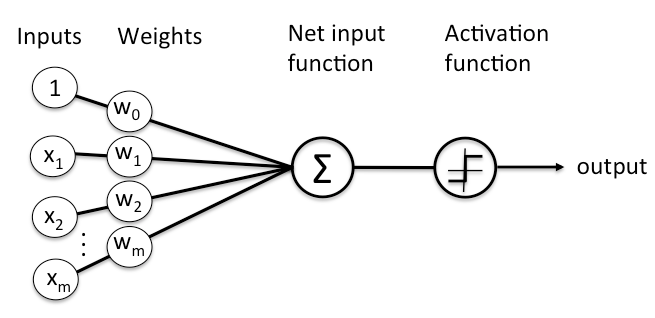
\includegraphics[width=1\textwidth]{artificial_neuron}
    \caption{\emph{Anatomy of an artificial neural network \cite{pathMind}}}
    \label{fig:artificial_neuron}
\end{figure}

The aforesaid \textbf{activation function} is a mathematical expression that helps
the ANN to add non-linearity to itself. With more and bigger datasets,
the patterns that need to be identified become more complex.
With the help of these types of function, the input is much easier to analyze and interpret.

\begin{itemize}
    \item{
          \textbf{zero-centered}: output should be symmetrical
          at zero so that it does not move to a particular direction;
          }
    \item{
          \textbf{computationally inexpensive}: the function is called for every layer
          for each input data, meaning that it could be invoked thousands of times.
          Therefore, they should not be computationally expensive;
          }
    \item{
          \textbf{differentiable}: at the core of almost every machine algorithm lies
          an optimization algorithm. One of the most popular
          approaches is the gradient descent algorithm in which one of the most essential
          features is that the function used needs to be differentiable;
          this idea will be discussed in detail in a subsequent paragraph;
          }
\end{itemize}



\subsection{Backpropagation and gradient descent}

\textbf{Backpropagation} describes how machine algorithms learn.
As shown in Figure\emph{\ref{fig:backpropagation}},
after the data traverses the neural network in a forward manner,
propagating the signals through the neurons,
the algorithm will go in reverse adjusting each weight for each node and its links \cite{Goodfellow-et-al-2016}.
This technique is called backpropagation of errors, or simply,
backpropagation and is the learning engine of the most ANN's.

\begin{figure}[h]
    \centering
    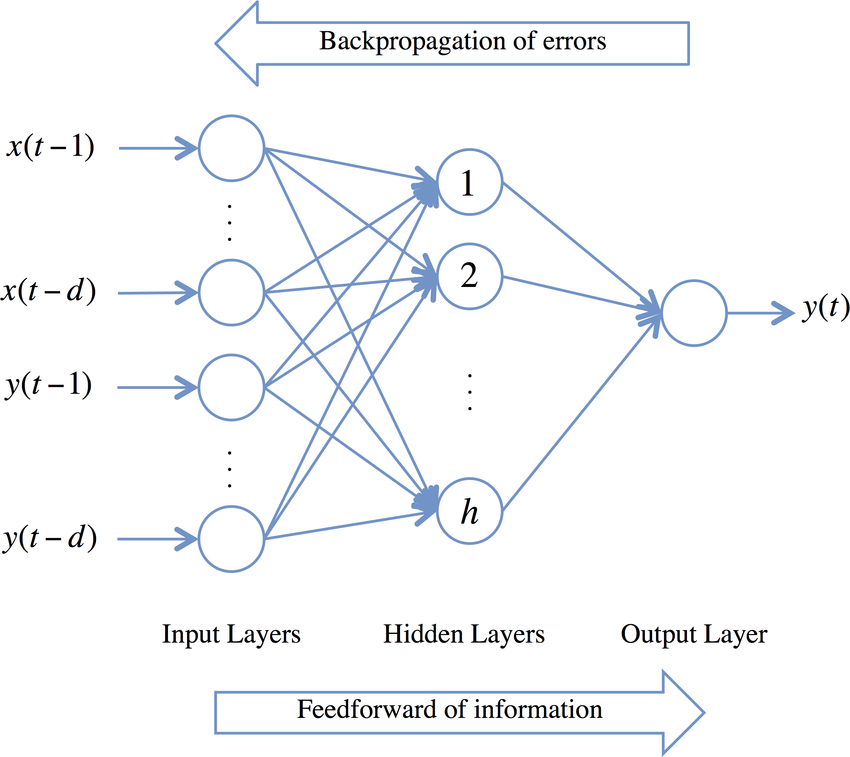
\includegraphics[width=1\textwidth]{backpropagation}
    \caption{\emph{Feedforward Backpropagation Neural Network architecture. \cite{backpropagation}}}
    \label{fig:backpropagation}
\end{figure}

The \textbf{gradient descent}, as mentioned before,
is an optimization algorithm best-used to find the (local) minimum value for a function \cite{brownlee2016master}.
Hence, it can be used to reduce the errors in our algorithm,
since the training of a neural network is just the process of finding the set of weights and other
parameters in such a fashion that the errors(differences) between our expected and actual results are minimum.
Hence, the gradient descent is used to compute the errors of our algorithm, that will be later backpropagated
through the ANN.


\subsection{Layers of ANNs}
Multiple artificial neurons are grouped in \textbf{layers};
the purpose of each one is to apply a non-linear
transformation of the input from one vector space to another \cite{appliedDeepLearning}.
As you can see in \emph{\ref{fig:ann_structure}} there are three types of layers in an artificial neural network:
\begin{itemize}[]
    \item{ Input layer
          \begin{adjustwidth}{1cm}{}
              This layer of a neural network is the very beginning of the ANN’s workflow, bringing the initial data into the system for
              further processing by subsequent layers of artificial neurons \cite{inputLayer}.
          \end{adjustwidth}
          }
    \item{ Hidden layer
          \begin{adjustwidth}{1cm}{}
              Any layer between the output and the input layer is considered to be a hidden layer.
              The number of neurons they contain and also their number can vary.
              Their role is to take in a set of weighted inputs and produce an output through an activation function \cite{hiddenlayer}.
          \end{adjustwidth}
          }
    \item{ Output layer
          \begin{adjustwidth}{1cm}{}
              This layer of a neural network is the last layer of neurons that produces given outputs for the program.
              They usually are made much like any other artificial neuron, but they may be observed in a different way,
              the output layer coalesces and concretely produces the end result \cite{outputLayer}.
          \end{adjustwidth}
          }
\end{itemize}
\begin{figure}[h]
    \centering
    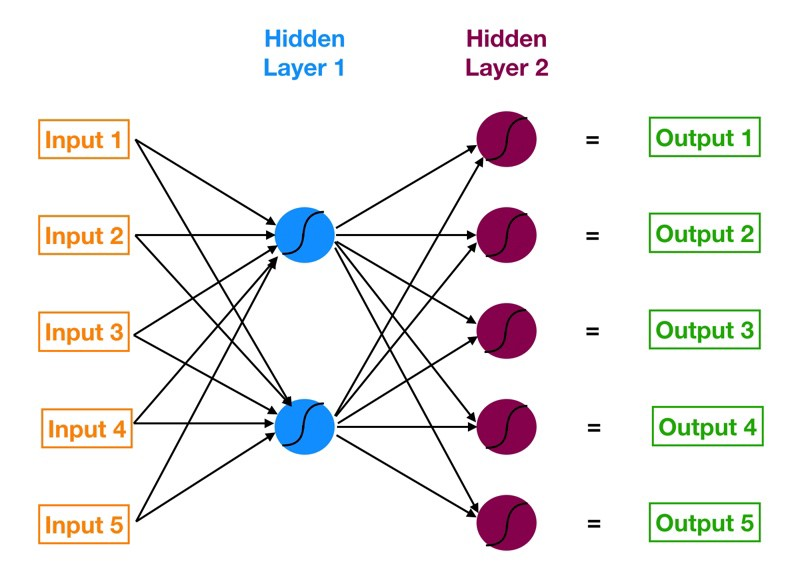
\includegraphics[width=1\textwidth]{ann_structure}
    \caption{\emph{Neural network with one hidden layer \cite{understandingANN}}}
    \label{fig:ann_structure}
\end{figure}


\section{What is Deep Learning?}

Deep learning is a subfield of machine learning that contains a collection of ANNs that are known for
their capability on learning unsupervised from data that is unstructured or unlabeled,
also known as deep neural learning or deep neural network.

A second classification we can make on ANNs is based on the relationships between their nodes.
Then, neural networks can be recurrent or feedforward;
the first one does not have any loops in its graph and can be organized in layers.
A deep neural network is a feedforward ANN with many hidden layers.

A visual representation of the aforementioned is the Figure\emph{~\ref{fig:deep_vs_normal}}
wherein we could see the differences between a simple feedforward ANN with one
hidden layer(left) and a deep neural network with three hidden layers.
\begin{figure}[h]
    \centering
    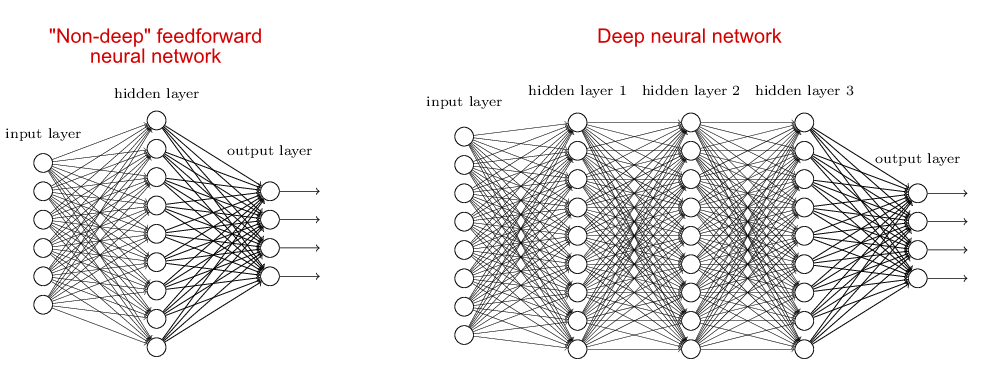
\includegraphics[width=1\textwidth]{deep_vs_normal_ann}
    \caption{\emph{Difference between a Non-deep ANN(left) and a deep ANN(right) \cite{deepLearningBook}}}.
    \label{fig:deep_vs_normal}
\end{figure}

Deep learning is an area in machine learning that achieves state-of-the-art
results by learning to represent the world "as a nested hierarchy of concepts,
with each concept defined in relation to simpler concepts,
and more abstract representations computed in terms of less abstract ones".\cite{Goodfellow-et-al-2016}

A visual representation of the aforementioned statement can be seen in Figure 2.3.



\section{Autoencoders and how they learn}

Autoencoders are neural networks usually used for dimensionality reduction.
They learn in an unsupervised manner,
their purpose being to obtain the internal representation of
the data by compressing and then reconstructing the original input,
making a copy of it.\cite{deepLearningBook}

This type of neural network is composed of two parts:

\begin{itemize}
    \item \textbf{encoder}
    \item \textbf{decoder}
\end{itemize}

The first one may be viewed as a network that aims to compress
our data into a  lower dimension code, named encoding.
It could be represented as a function \(\boldsymbol{h}=f(x)\).\cite{deepLearningBook}

The second one intends to reconstruct the input based on that encoding,
removing thus all the possible noise.
It could be represented as a function \(\boldsymbol{r}=g(h)\).\cite{deepLearningBook}

\begin{figure}[h]
    \centering
    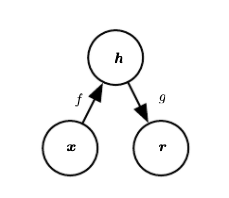
\includegraphics[width=0.4\textwidth]{autoencoder}
    \caption{\emph{Structure of an autoencoder \cite{deepLearningBook}}}.
    \label{fig:autoencoder}
\end{figure}

Therefore, as shown in Figure \ref{fig:autoencoder},
the entire autoencoder can be seen as the following function: \(g(f(x))=x\).
In other words, an autoencoder tries to mimic the identity function,
but, due to the compression, is unable to do so.
However, thanks to that same compression,
it learns how to successfully identify
the most important features of our data's internal structure,
represented by the encoding.


% \end{justify}

\chapter{Music and Machine Learning}
Music, one of the oldest forms of art and entertainment humanity has ever had,
has played a significant role in different cultures and civilizations worldwide
since the beginning of history.

With the progress of artificial intelligence in many areas such as computer vision,
speech recognition, and natural language processing,
machine learning enthusiasts have tried
to use all their knowledge in music-related fields. \cite{musicCompositionML}

Artists tried different approaches to music composition,
from free playing and improvisation to diving deep into the
rhythm, notes, scales, modes, and other elements of music theory,
for both of them existing various approaches in machine learning.
This chapter explores several of these methods related to this paper's work,
but before immersing in the machine learning aspects, we should discuss how they process data.



\section{What is MIDI?}
MIDI (\textbf{M}usical \textbf{I}nstrument \textbf{D}igital \textbf{I}nterface) specifies a standard for connecting,
playing, and recording electronic instruments and a file format to store this information.
It uses messages in an event-driven manner,
meaning that each note is represented as an event that specifies its
notation, pitch, velocity, and other useful characteristics. \cite{midiCourse}

The MIDI file format is a popular choice among data scientist
when working with audio and music due to several aspects:

\begin{itemize}
    \item{
          \emph{ease of manipulation}:
          one can edit the parameters of a note without the need for rerecording; \cite{midiAmanda}
          }
    \item{
          \emph{ability to change instruments}:
          a MIDI file only defines what notes should be played and in which order,
          not the instrument that should perform them; \cite{midiAmanda}
          }
    \item{
          \emph{small size}: this file format is comparable to an electronic sheet;
          it does not hold any audio information,
          only instructions for playing the notes,
          saving a whole song in just several kilobytes of data. \cite{midiAmanda}
          }
\end{itemize}

\section{LakhNES and Transformer-XL}

One of the latest music-generation approaches is Chris Donahue's
\emph{LakhNES: Improving multi-instrumental music generation with cross-domain pre-training}.
The author uses language models and their ability to retain long-term sequences within the data,
being able to generate multi-instrumental structured songs. \cite{donahue2019lakhnes}


Before discussing his approach,
one must understand the insights of the used models.
Transformer-XL is a neural network used for resolving natural language processing tasks,
achieving state-of-the-art results on different language datasets.
Other proposals for these problems are models based on recurrent neural networks and long
short-term memory, which give great results on more straightforward data,
but cannot establish longer dependencies between words due to their limitations. \cite{transformerXLMedium}

\begin{figure}[h]
    \centering
    \includegraphics[width=1\textwidth]{Transformer_XL}
    \caption{\emph{Transformer-XL - training and evaluation \cite{transformerXLMedium}}}
    \label{fig:transformerXLMedium}
\end{figure}

Vanilla Transformers tend to resolve this problem by introducing new attention modules.
They receive a sequence of tokens (instead of processing tokens one by one)
and determine the connections between them based on absolute positional encoding.
The main obstacle with this network is that it can only receive
one sequence of specified length at a time;
hence, the data can suffer from context fragmentation. \cite{transformerXLMedium}


\begin{wrapfigure}{L}{0.5\textwidth}
    \centering
    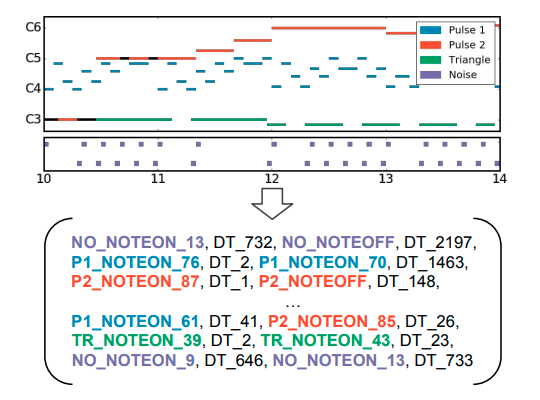
\includegraphics[width=0.45\textwidth]{lakhnessConversion}
    \caption{\emph{Note conversion example used in \cite{donahue2019lakhnes}}}
    \label{fig:noteConversion}
\end{wrapfigure}

Transformers-XL solves the problems mentioned above by
using relative positional encoding and a recurrence mechanism
to extend their context for much better and faster performance.
Figure\emph{~\ref{fig:transformerXLMedium}} represents a small outline of the training and evaluation phase of the discussed network,
in which one can observe how the extended context is created and used.




In \cite{donahue2019lakhnes}, they used the Transformer-XL,
by creating a grammar through which they converted the MIDI events
into text that the network can process.
An example of this conversion is in Figure\emph{~\ref{fig:transformerXLMedium}}.
In this manner,
they can convert any MIDI to some text with
which they train the model and then use it
for generating new complex structured songs or
completing existing ones.


Another noticeable aspect of their work is that they used
transfer learning, their purpose being to generate NES music game,
but, by using this approach of pre-training their model with
general standard data, they increased the performance of the model
by 10\%. \cite{donahue2019lakhnes}


\section{Composer and Autoencoders}
The main inspiration for this work is HackerPoet's \emph{Composer} \cite{hackerPoet},
another point of view for music generation that uses deep autoencoders.

As explained in the previous chapters,
this type of neural network learns in an unsupervised manner the internal representation of our data.
Using only the decoding part,
the author generates new MIDIs by feeding it new normalized encodings and predicting new songs.
He trained his model with game music utilizing a dataset that he created, his main goal being game themes. \cite{hackerPoet}

This approach has excellent results regarding music theory,
the model being able to compose songs with a well-defined structure,
having popular chord progressions, bassline, multiple melodies, and also musical motifs. \cite{hackerPoet}

The good results and the ease of understanding and implementing autoencoders are
the main reason they have been used in this application, one key difference in this paper's
approach being represented by the structure of our autoencoder and how the encoding was
enhanced with the emotional value from the dataset.


\section{AIVA - Artificial Intelligence Virtual Artist}

Another proposal worth mention is the algorithm behind the startup \emph{AIVA} \cite{aiva}.
It is a deep learning model that uses reinforcement learning,
initially and mainly trained on classical pieces based on compositions of great musicians
like Mozart, Beethoven, and Bach.
In the latest releases, it was also trained on different styles of music. \cite{aiva1}

It is the first artificial intelligence recognized as a composer by a copyright authority -
SACEM (standing for Society of Authors, Composers and Publishers of Music).
Therefore, its pieces are not public, their songs being copyrighted. \cite{aiva2}

AIVA's algorithm most essential features are creating new compositions or
finishing existing ones based on a given genre, or even writing with influences of another song.
In other words, it can learn the style of a piece and compose a song
in the same fashion as the input one.\cite{aiva1}


\chapter{Proposed approach}
\section{Problem definition}
With the advancements of technology,
people tried digitalizing every aspect of their life.
They renounced the traditional slow postal services in favour of
the modern fast email.
Digital photos gained popularity to the detriment of physical copies.
In the same way, CDs and other physical mediums were
forgotten with the arising of digital MP3s.


Over the past years, with the rise of the Internet,
even the idea of digitalizing one's life became old,
so people started to sync it with the cloud.
Hence, a new way of storing and transmitting data emerged: streaming.

\begin{figure}[h]
      \centering
      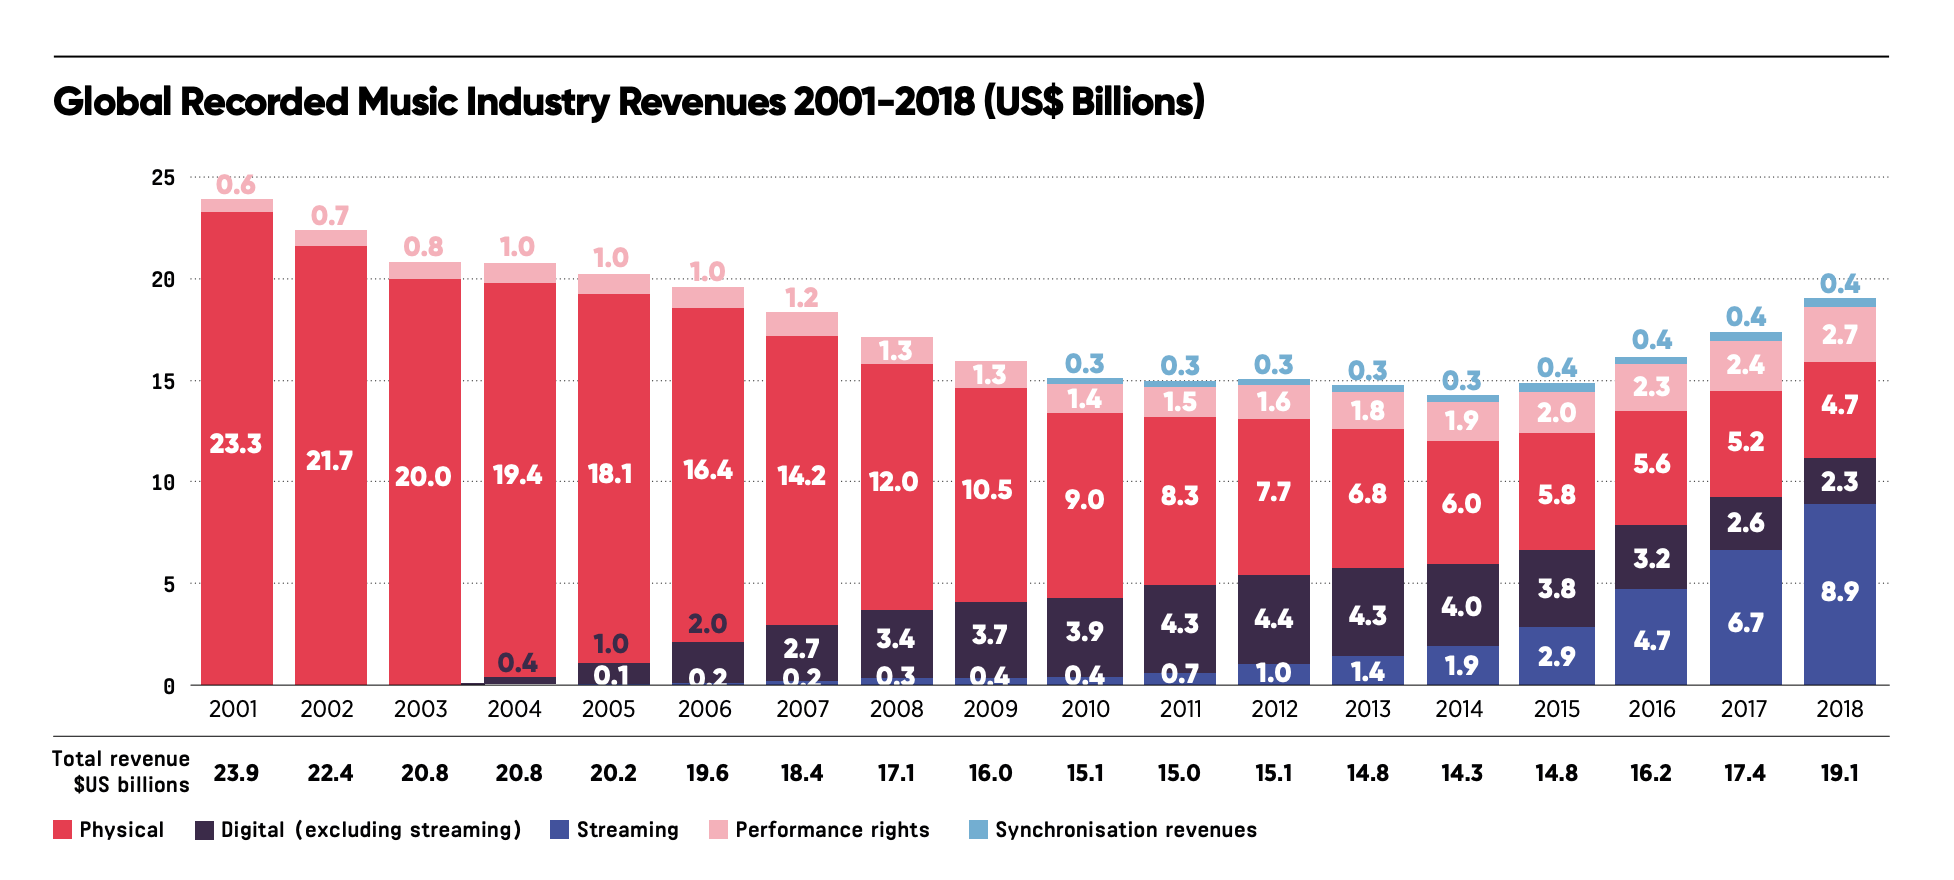
\includegraphics[width=1\textwidth]{ifpi}
      \caption{\emph{Global Recorded Music Industry Revenues 2001-2018  \cite{ifpi}}}
      \label{fig:ifpi}
\end{figure}

As shown in Figure\emph{~\ref{fig:ifpi}}, in the last decade,
the revenue of the music industry shifted,
going from physical to digital; nowadays,
the highest income is generated by streaming means.

With this change, one can easily compose and produce
music from their studio or even bedroom,
since it is not compulsory to be tied to a record label.
There are lots of successful independent musicians who
create music this way and the numbers are growing more
and more every year \cite{forbes}.

Even with all these developments,
the act of composing music did not drastically change in the last
few hundred years. If one wants to compose a song,
they should learn how to use instruments,
and how to put notes in such a manner that they sound good together.
Technology eased the process of composing,
but one must still learn chords, scales,
and other elements of music theory to make the process less hazardous.
Although music theory has a steep learning curve,
learning it helps express oneself musically.
Despite all these advancements,
there is a lack of tools facilitating the creative process.

This paper tries to fill the aforementioned deficit;
with the help of machine learning,
it proposes a system whose goal is to aid the aspiring musician easily
compose a song based on a given emotion.
It provides a way of generating new pieces of music without the need to master music theory.


\section{Orpheus's Sorrow's Approach}
\emph{Orpheus's Sorrow} is the name of the system mentioned before.
It is a client-server web application where a musician can input
emotion data and values to other parameters to visualize songs that this deep
neural network generated on the given data.
In the following sections,
we will discuss the paper's approach related to music and emotion,
dataset creation, and the internal structure of the model.


\subsection{Music, emotions and machine learning}
\begin{wrapfigure}{L}{0.5\textwidth}
      \centering
      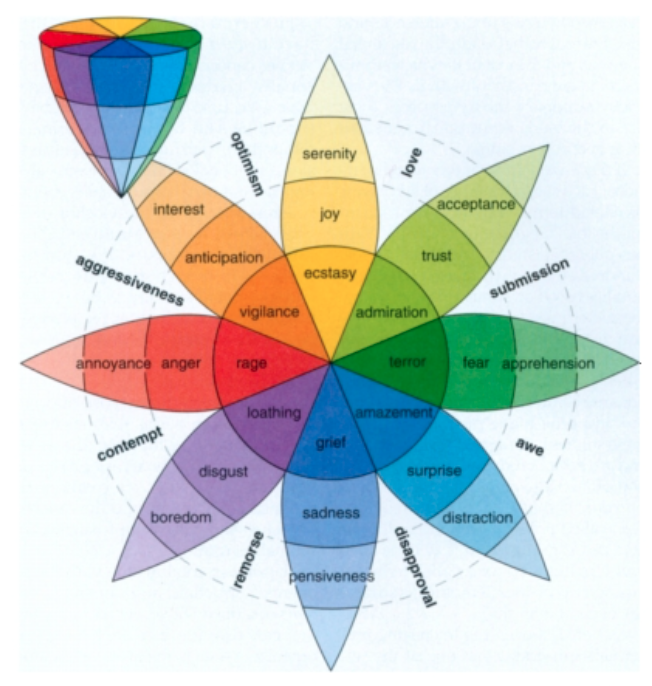
\includegraphics[width=0.45\textwidth]{plutchik}
      \caption{\emph{Plutchik's wheel/cone of emotions \cite{plutchik}}}
      \label{fig:plutchik}
\end{wrapfigure}
Music and emotion are highly connected,
one of the main goals of a composer being expressing his feelings through notes,
trying to reach his audience, and to induce them his mood and ideas.


When dealing with music classification based on the emotion it expresses,
there are multiple strategies for managing the sentiment data,
the most popular being tag-classification using some predefined emotions
or a regression approach representing the feeling through some variables.
Both of the approaches can be applied to the whole song or a subset of
features extracted manually or automatically.


The first one usually is paired with an existing model for emotions,
one of the most popular being Plutchik's wheel of emotions.
As can be seen in Figure\emph{~\ref{fig:plutchik}},
Plutchik circularly arranged the feelings,
proposing eight primary bipolar emotions:
surprise - anticipation, fear - anger, trust - disgust, joy - sadness.


\begin{wrapfigure}[10]{r}{0.5\textwidth}
      \centering
      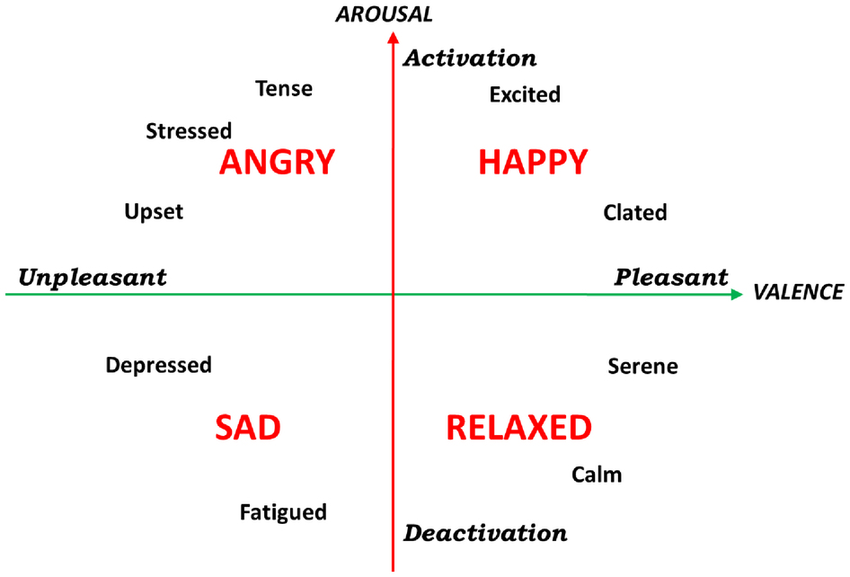
\includegraphics[width=0.45\textwidth]{thayers}
      \caption{\emph{Thayer's Model for Emotions (also named Russel's model) \cite{plutchik}}}
      \label{fig:thayers}
\end{wrapfigure}

When choosing the second, one frequently uses Thayers's
(also called Russell's) model. With this method,
every emotion can be described using two variables: valence and arousal.


As seen in Figure\emph{~\ref{fig:thayers}}, in this way,
feelings can be plotted on a cartesian system of coordinates obtaining
four general quadrants of emotions: happy, angry, sad, and relaxed.

\vspace{1cm}


\subsection{MIDIs and Emotion Dataset}

\begin{wrapfigure}[13]{l}{0.5\textwidth}
      \centering
      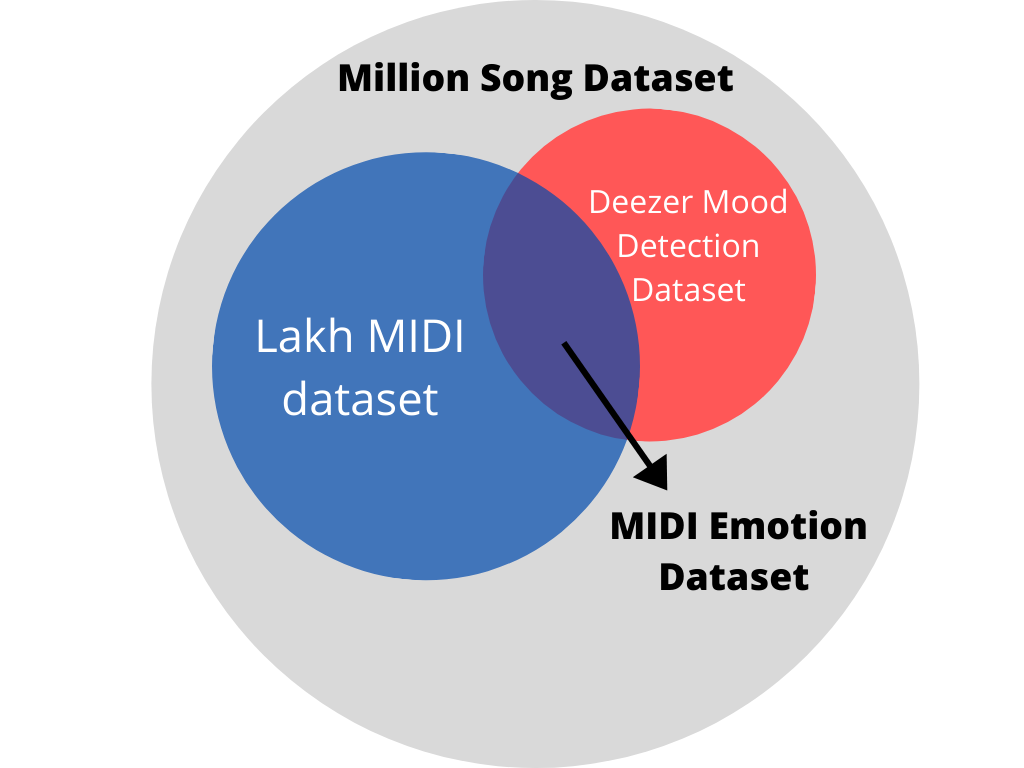
\includegraphics[width=0.45\textwidth]{dataset_creation}
      \caption{\emph{Merging existing datasets to create a new one}}
      \label{fig:dataset_creation}
\end{wrapfigure}

When discussing machine learning and neural networks,
one must know what data is available for their needs,
how to parse their data in a format they fully understand and maximizes
the potential of their data.

The model proposed uses MIDIs to store and handle the music information
data due to ease of manipulation, as mentioned before.
During quick research, there were not any free/public datasets
that satisfied the needs of the problem statement - a
dataset containing MIDIs with the emotion value(arousal and valence)
attached to each song. Hence there was a need to create a new dataset
by merging some of the existing ones to fulfill the requirements.
The merged datasets are the following:
\begin{itemize}
      \item{
            \textbf{Million Song Dataset} - a free compilation of metadata for a million contemporary common music records;\cite{themillion}
            }
      \item{
            \textbf{Lakh Midi Dataset} - set of over 150,000 unique MIDI files, over 40,000 being matched to entries in the dataset mentioned above;\cite{lakh}
            }
      \item{
            \textbf{Deezer Mood Detection Dataset} - valence and arousal dataset for over 10,000 songs also matched to the first-mentioned dataset.\cite{deezer}
            }
\end{itemize}



A visual representation of the sets is in Figure \emph{\ref{fig:dataset_creation}}.
It represents how the merging was performed.
The songs from the last two datasets were paired based on their
ID in the Million Song Dataset and then joined together with their relevant information.
The new dataset contains over 1800 MIDIs, with their respective valence and arousal,
enough data to train the model to see if this approach can have good results.

The obtained dataset was split into three parts: 80\% training data,
10\% validation data, 10\% testing data.
The training data was also augmented by shifting the pitch with several notes higher and lower.

\subsection{Model architecture}
Now, with the data ready to be fed to the model,
in the following paragraphs,
it will be discussed about its sampling and also about the structure of the model.

Feeding the MIDI file directly in the model
will not produce good results since there are too many irrelevant pieces of information
beyond our purpose, and that will confuse the network.
Before the actual training of the MIDI,
the files were transformed into piano rolls,
being sampled as a set of images.
A piano roll here consists of an image of type $noteRange * timing$.
The latter was chosen as 96, as used in \cite{hackerPoet},
mainly because almost all standard time signatures are dividing.
For the first one is chosen the same value since very few songs use the highest
and lowest pitches and also for symmetry's sake.

\begin{figure}[h]
      \centering
      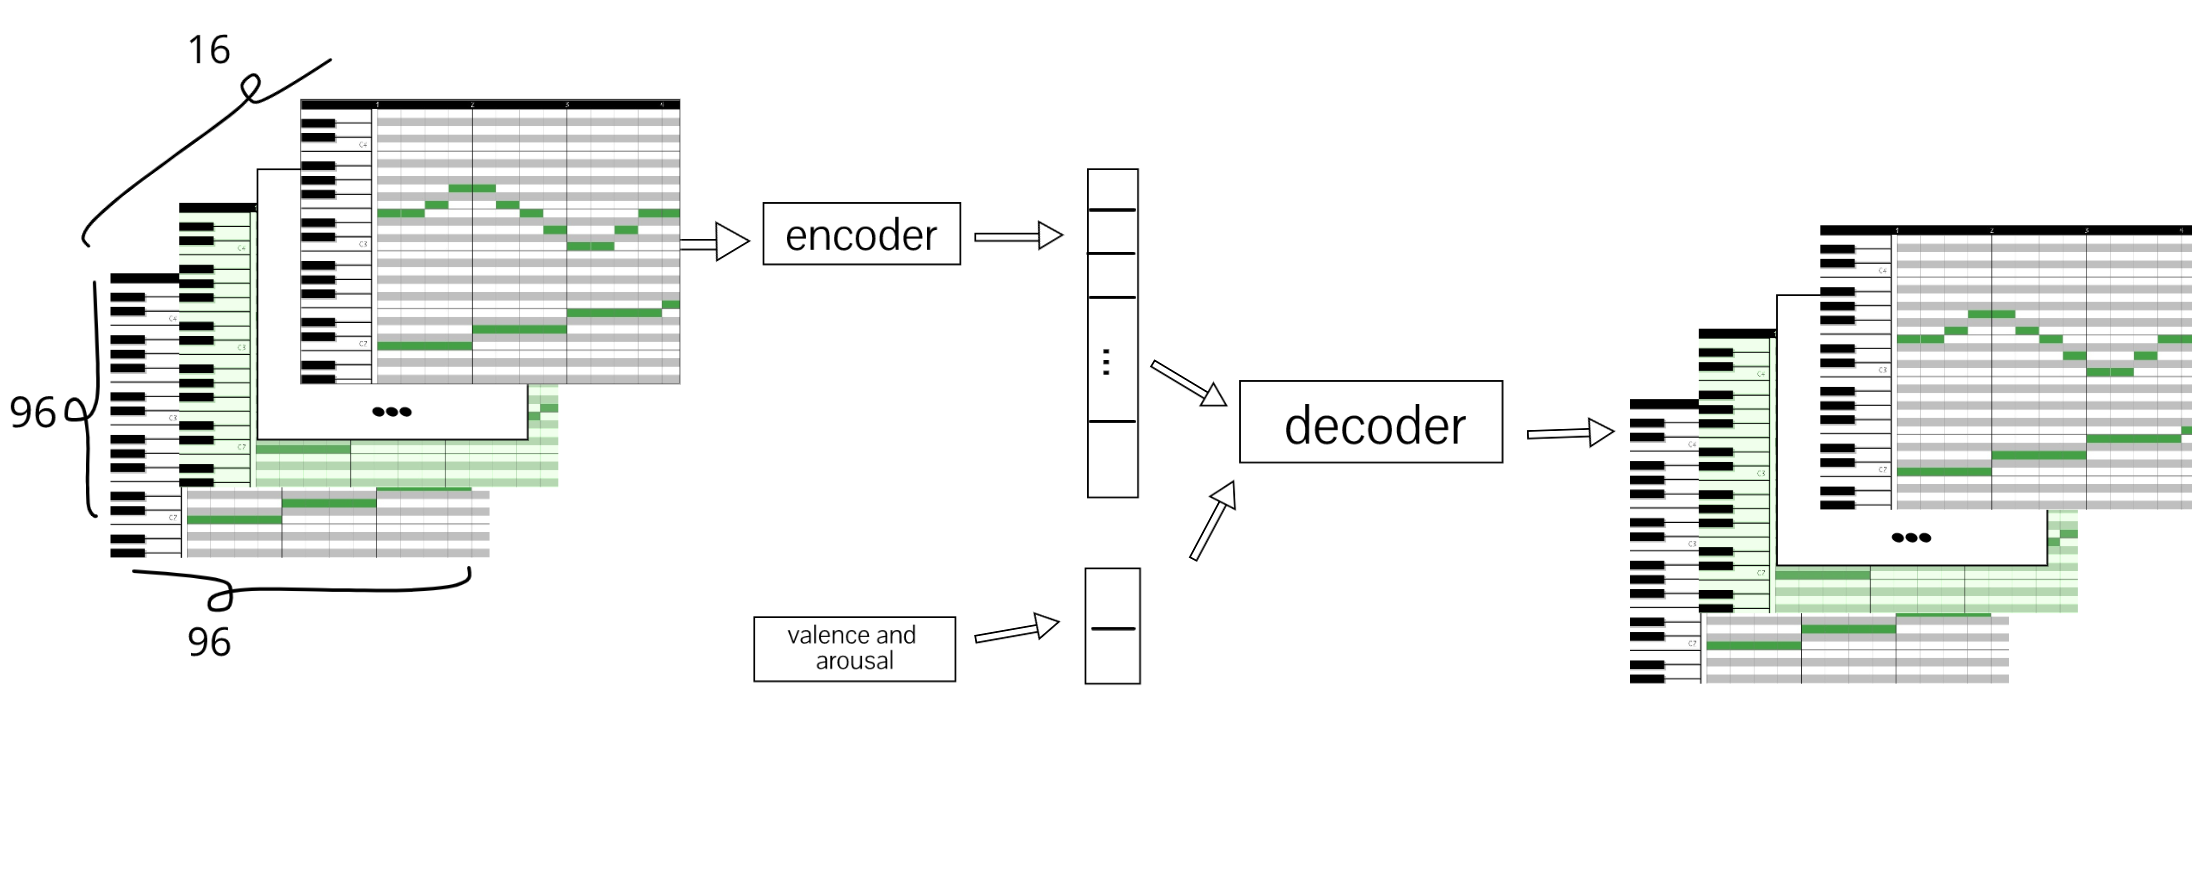
\includegraphics[width=1\textwidth]{model_short}
      \caption{\emph{Short description of paper's model}}
      \label{fig:model_short}
\end{figure}

As seen in Figure \emph{\ref{fig:model_short}},
the deep neural network consists of a deep autoencoder used to find the encoding of a song;
in other words, it finds the essential features of that piece of music.
It works similarly with the \cite{hackerPoet},
but the main highlight of this particular model is that to its encoding
are concatenated the valence and arousal values for each song,
this approach helping it to learn how to generate songs based on its input emotion data.

The composing works by creating an auxiliary model,
namely a Keras backend function,
that represents the decoder.
Its input is represented by two arrays,
the 48 values for the features the network identified,
and the emotional values; the set of piano rolls represents its output,
generating in this manner a new song.

Next, the main structure of the model will be presented,
with its primary layers and other parameters configured, as depicted in Figure \emph{\ref{fig:model}}.


\begin{figure}[H]
      \centering
      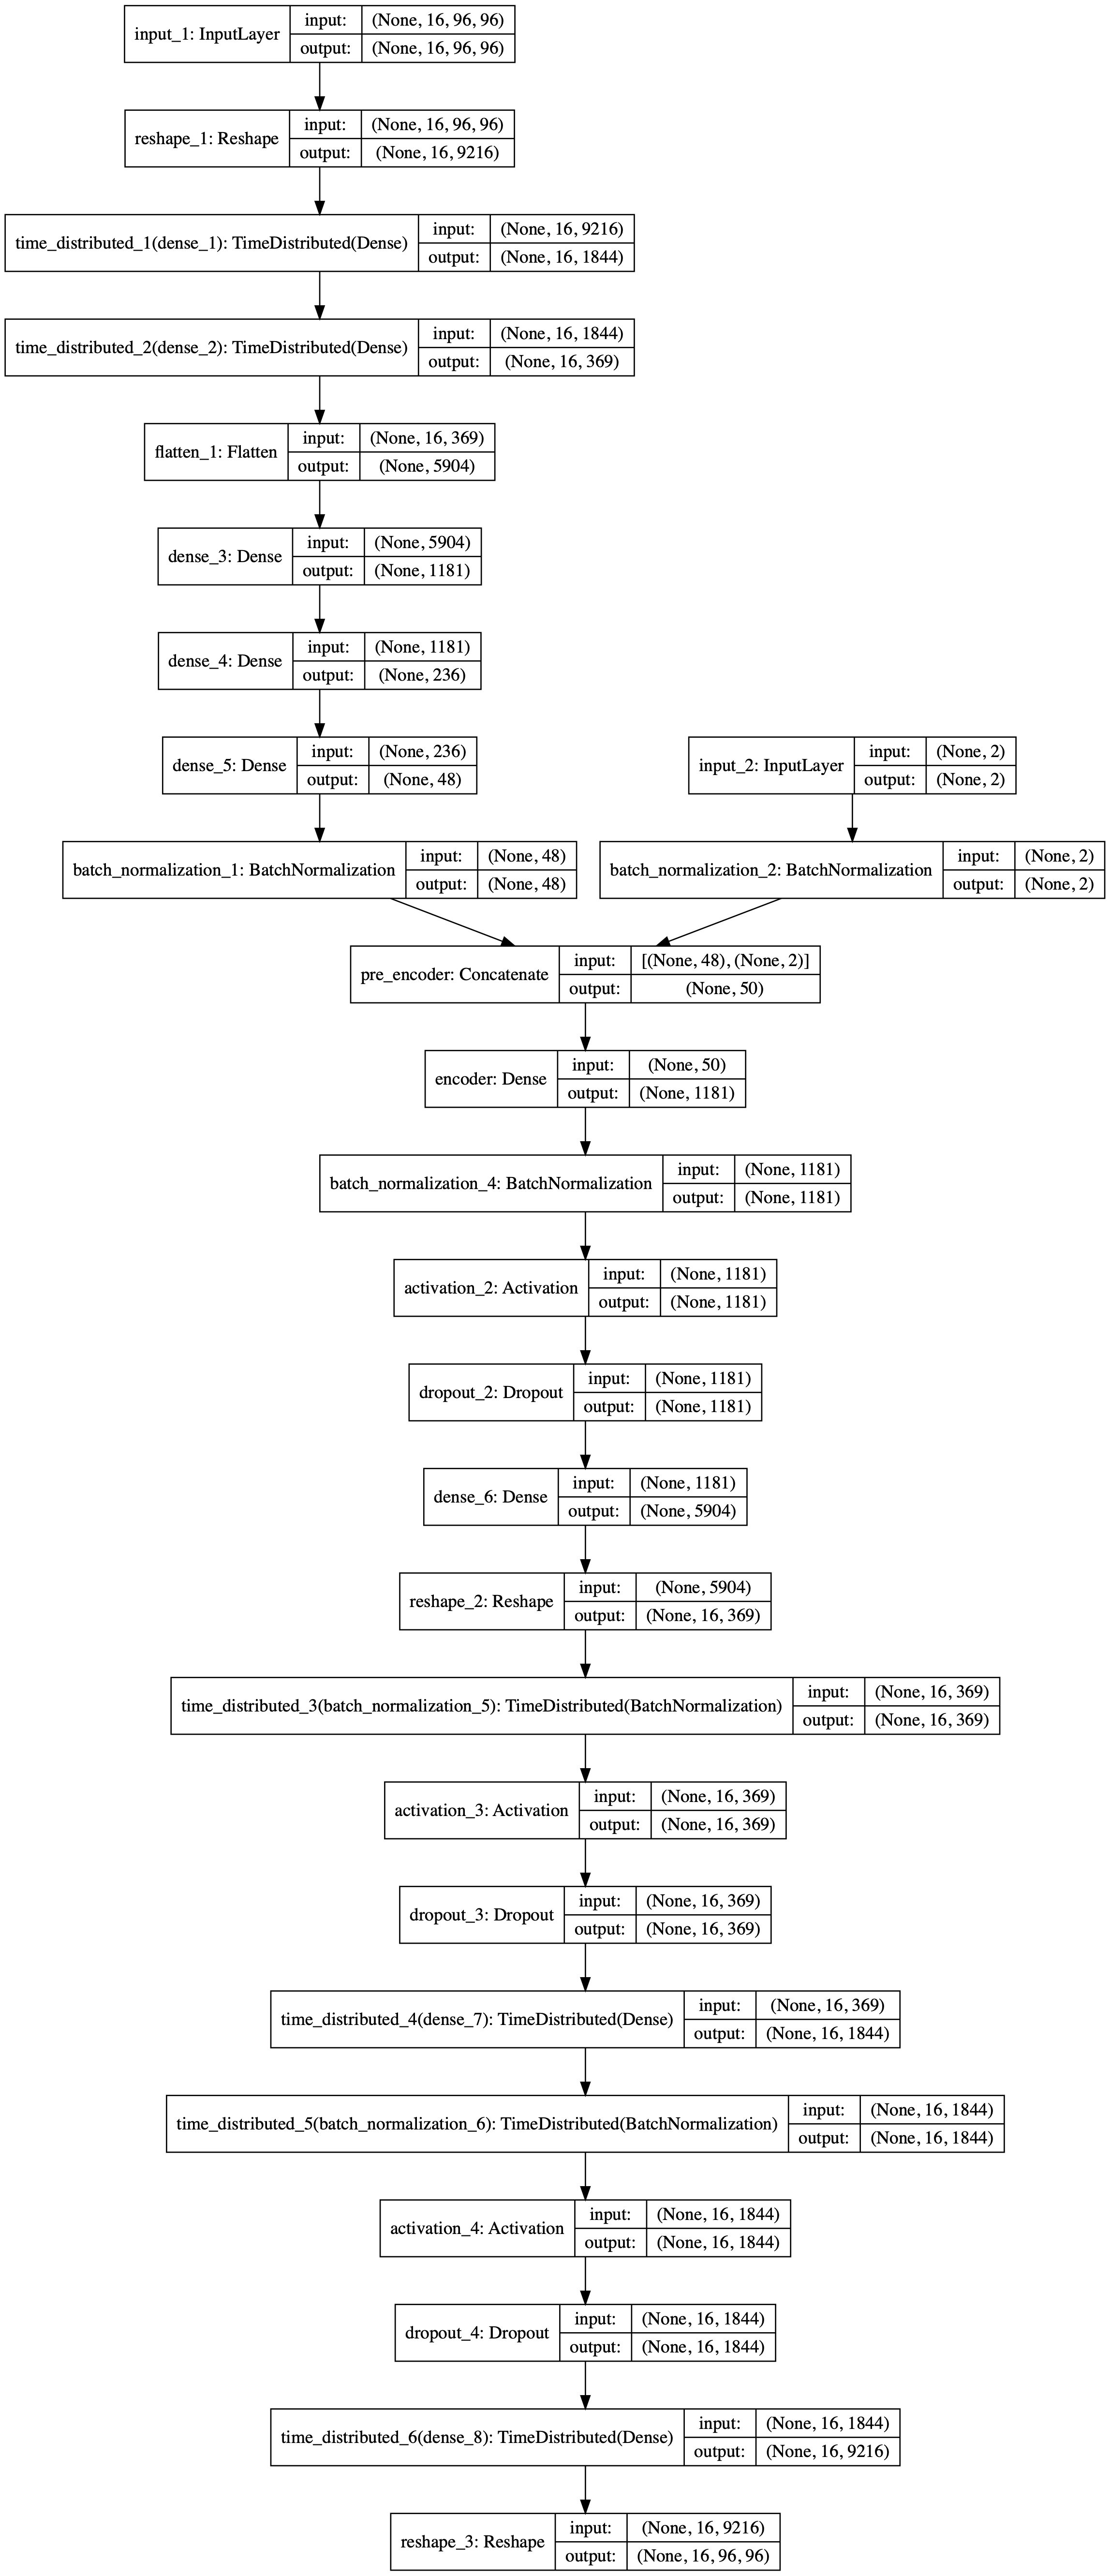
\includegraphics[height=0.8\paperheight, width=1\textwidth]{model}
      \caption{\emph{Structure of the model}}
      \label{fig:model}
\end{figure}

For increasing its stability and speed, the model uses the batch-normalization layers.
Their purpose is to normalize the output of the prior activation layer
by subtracting the batch mean and dividing by its standard deviation,
reducing in this manner generalization errors, providing some regularization. \cite{batchNorm}


Another vital layer that helps to group the rolls in time-based sets is the time-distributed layer.
It is usually used as a middleware for 3D input; given a timestep,
it applies the same layer it wraps to each temporal slice of the same size as the timestep.\cite{keras}

\begin{wrapfigure}[8]{L}{0.5\textwidth}
      \centering
      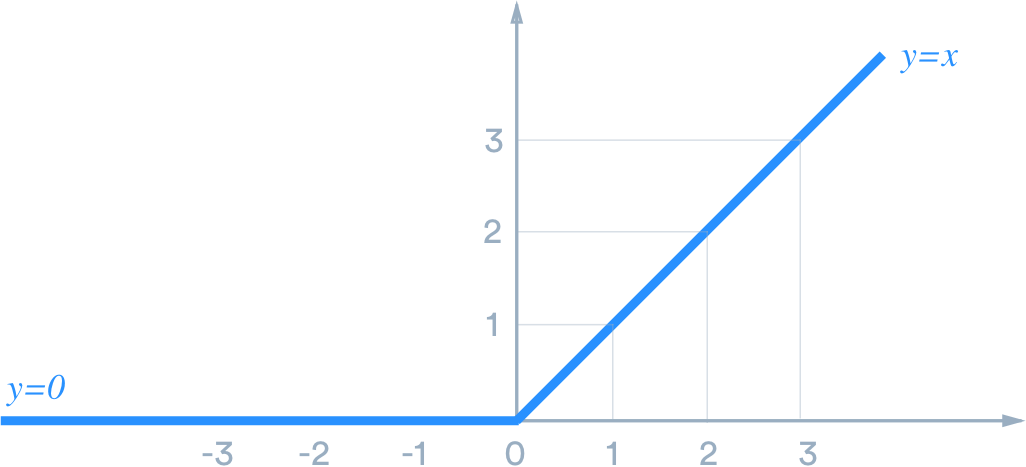
\includegraphics[width=0.3\textwidth]{relu}
      \caption{\emph{ReLU visual representation \cite{relu}}}
      \label{fig:relu}
\end{wrapfigure}

Another characteristic of our model is the activation function used -
ReLU(Rectified Linear Unit). Figure \emph{\ref{fig:relu}} represents the function mentioned before,
expressed mathematically as $y = max(0, x)$. It is not expensive to compute,
the model taking less time to train and run. \cite{relu}

The loss function used is the binary cross-entropy since the model
has to predict the probability of playing or not a note in its current context,
the mentioned function being the default used in binary classification problems.\cite{cross}


\subsection{Loss and Accuracy}


\begin{figure}[h]
      \centering
      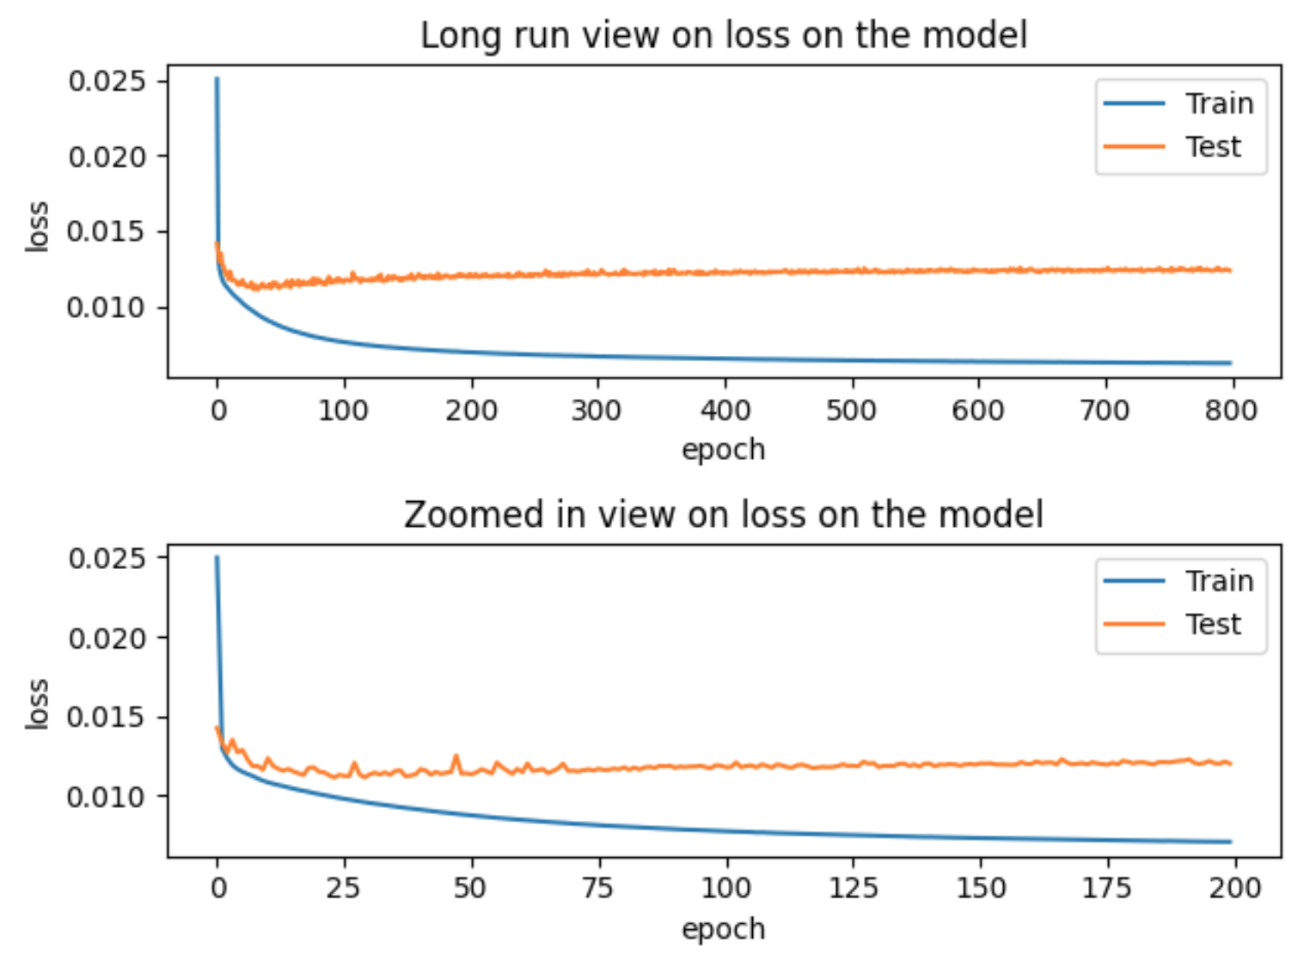
\includegraphics[width=.8\textwidth]{loss}
      \caption{figure}{\emph{Visual representation of loss}}
      \label{fig:loss}
\end{figure}

Researching other approaches for music composition influenced this paper,
even regarding the number of epochs one should train the model.
There are various empirical ways to estimate the most suitable number of epochs,
but since our dataset has not been used in other machine learning algorithms,
or since it does not have a large number of MIDIs, when training,
the model uses a callback that saves the model every n-th epoch.
In this manner, the training period cannot be ruined by overfitting
since the model can be reloaded at any saved moment.


From each model saved,
there can be retrieved some metadata about our songs.
This new information will be used when generating another song,
normalizing the given input through singular value decomposition,
reassuring that our features are in the normal range of our data.


As can be seen in Figure \emph{\ref{fig:loss}}, the top part, in the long run,
the model starts overfitting around the 200-300th epoch,
statement tested by the fact that every model above that period starts
composing the same songs regardless the input data. On the zoomed-in view,
the bottom part of the same Figure, the slope stats getting smaller around 175-200th epoch,
the model that was empirically chosen the best being the 190th epoch
due to its ability to compose the most exciting songs with a well-defined structure,
and other essential characteristics such as constant rhythm,
repeating structures (motifs). The accuracy curve, as seen in Figure \emph{\ref{fig:accuracy}},
starts flattening nearby the same interval for the train data and becomes
constant almost for the validation data.
When evaluating the chosen best model on the 10\% songs from the dataset
it was not trained with, the result obtained is 98\% accuracy.


\begin{figure}[h]
      \centering
      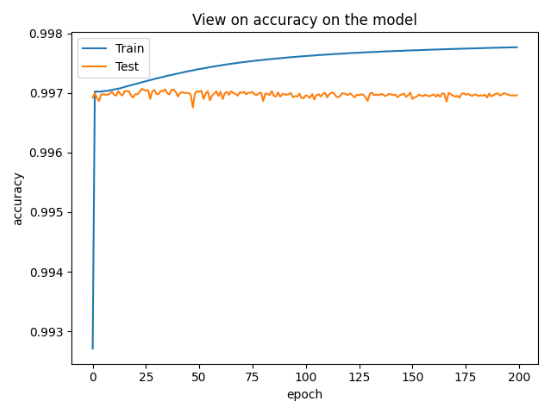
\includegraphics[width=.8\linewidth]{accuracy}
      \caption{\emph{Visual representation of accuracy}}
      \label{fig:accuracy}
\end{figure}



\section{Composing songs}
The discussed model, trained on the created dataset,
has excellent results regarding accuracy and loss,
but the generated songs do not get the same expected results regarding the emotion part.
Due to the smaller number of samples,
the learned features and also the valence and arousal values are very dependent,
meaning that given a composed song, at first listen,
the emotion denoted by the song is not clear, in the majority of cases.

Despite the vague emotion a composed song induces,
there are some characteristics that the model learned for each different quadrant
(see Figure \emph{\ref{fig:thayers}}).
For the first one (happy), most of the songs are using the major scale,
the most common characteristic of a happy song.
For the second one (angry), a preponderance of the songs is using minor scales,
part of them also tritones/dissonant chords,
the note density over time is much bigger,
the rhythm being galloping;
all of the above are features more frequently encountered in angry songs.
The fact that most of the MIDIs in the dataset from the last-mentioned quadrant
are metal or classical songs is also notable.
For the third quadrant (sad), a part of songs uses minor scales,
this being the quadrant with the most ambiguous results.
For the last quadrant (relaxed), some songs also use the major scale,
but the most notable fact is the low density of notes,
which is characteristic of slow-paced, calm songs.



\chapter{Application}

This chapter will present the client - server application in which the model is utilized,
the technologies used, main use cases/features,
and the app's design and implementation.


\section{Technologies used}

Before discussing other implementation and design details,
this section will present the technologies and tools used in this paper's
application and model.

\subsection{Keras}
Keras is an intuitive API for creating deep neural networks,
whose aim is to reduce the cognitive load.
It makes one able to focus on the data,
but still being able to obtain state-of-the-art results, being used by NASA,
CERN, and many more scientific organizations due to its flexibility,
but also by the top-5 winning teams on Kaggle, due to its speed of iterations,
letting one run experiments much more straightforward.\cite{keras}

\subsection{Flask}
Flask is a WSGI web application framework designed for an easier and quicker start,
but can also scale up to complex applications,
becoming one of the most popular Python web application frameworks.\cite{flask}

Flask does not demand any dependencies,
leaving it up to the developer to choose,
based on their needs, the tools and libraries they want to use. .\cite{flask}

\subsection{React}
React is a virtual-dom javascript library used for developing user interfaces.
It is declarative, making it more manageable to create interactive UIs,
designing simple views for each state of the application,
React efficiently updating,
and re-rendering the minimum number of components when the data changes.
Being declarative views it makes the code more predictable and more comfortable
to debug.
It is component-based,
allowing encapsulating simpler components then compose them into complex UIs.

\begin{figure}[H]
  \centering
  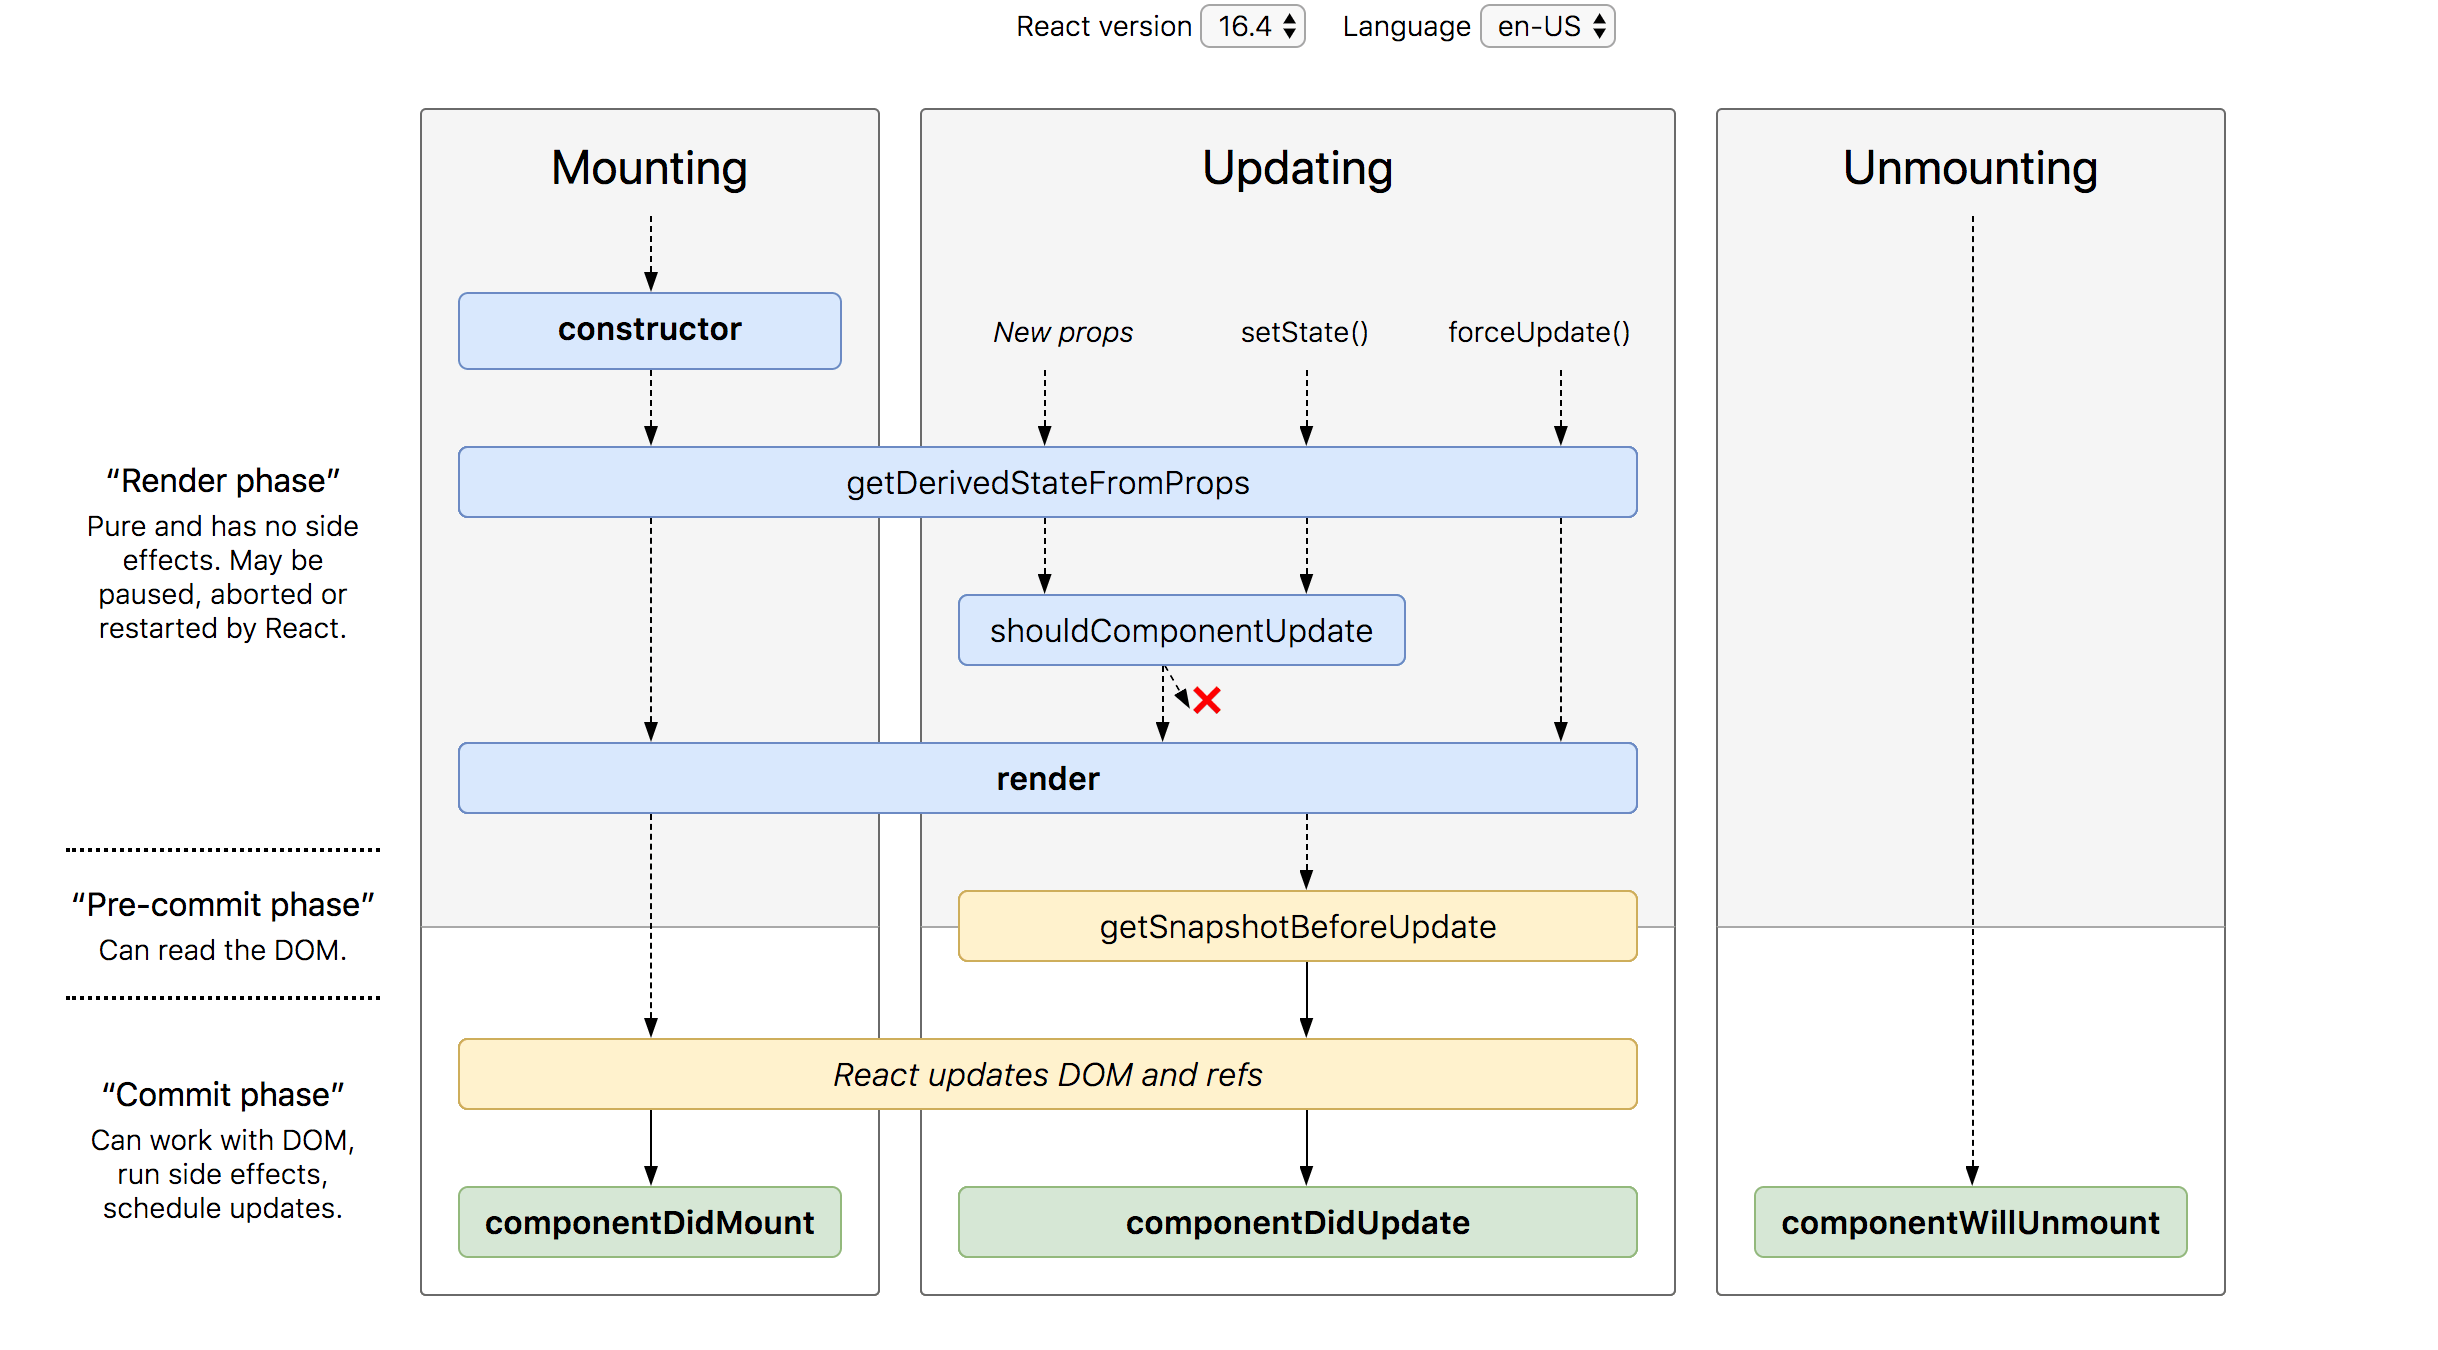
\includegraphics[width=.8\textwidth]{lifecycle}
  \caption{\emph{Lifecycle of a React Component}}
  \label{fig:lifecycle}
\end{figure}

Each created component is extending the React Component class
and should implement the render function.
It takes the input data and returns what to display.
Each component has two types of input data, which, when modified,
trigger re-rendering: props or external properties, and state or internal properties.
The rendering process is described as a lifecycle,
with a series of predefined steps,
some of them having a method that can be overridden
for a better manipulating of the UI, as seen in Figure \emph{\ref{fig:lifecycle}}.

\subsection{MobX-state-tree}
Mobx-state-tree (MST) is a state management library whose purpose
is to combine the traceability of immutable data with the simplicity
and ease of mutable data, also using the reactiveness
and performance of observable data.
The central concept of MST is the living tree.
It is an observable container data structure that consists of mutable data,
from inside the tree, using some defined methods, called actions,
from which are automatically generated immutable objects, called snapshots.
For developing the app, MST was chosen over other state management alternatives
(Redux, Flux, Recoil) thanks to its ease of writing,
lack of boiler code, and reactiveness of observable data.


\section{Main use cases/features}
In the following section,
there will be presented the main use cases of our application,
as depicted in Figure \emph{\ref{fig:usecase}}.
The main features/use cases of the app are the following:
\begin{itemize}
  \item{
        \emph{Generate song}: the musician should be able to input values
        for valence and arousal, and the app should respond with a composed song,
        that induces the corresponding emotion.
        \begin{itemize}
          \item actor: musician
          \item precondition: inputs for valence, arousal, and other model's features
          \item postcondition: a new song is generated and displayed to the user's browser
          \item path: the user should open the application, insert the input data, and the app would render the song it generated
        \end{itemize}
        }
  \item{
        \emph{See live edits of a song}: the musician should be capable of modifying the input and see live edits of the displayed song
        \begin{itemize}
          \item actor: musician
          \item precondition: a song generated before
          \item postcondition: UI is updated with the new form of the song
          \item path: the user should first generate a song then modify the input variables, and the app would render the new updated song
        \end{itemize}
        }
  \item{
        \emph{Listen to songs}: the user should be able to listen to the generated song
        \begin{itemize}
          \item actor: musician
          \item precondition: a song generated before
          \item postcondition: the application will start playing the generated song
          \item path: the user should first generate a song then press space bar, and the app would play the song
        \end{itemize}
        }
\end{itemize}

\begin{figure}[H]
  \centering
  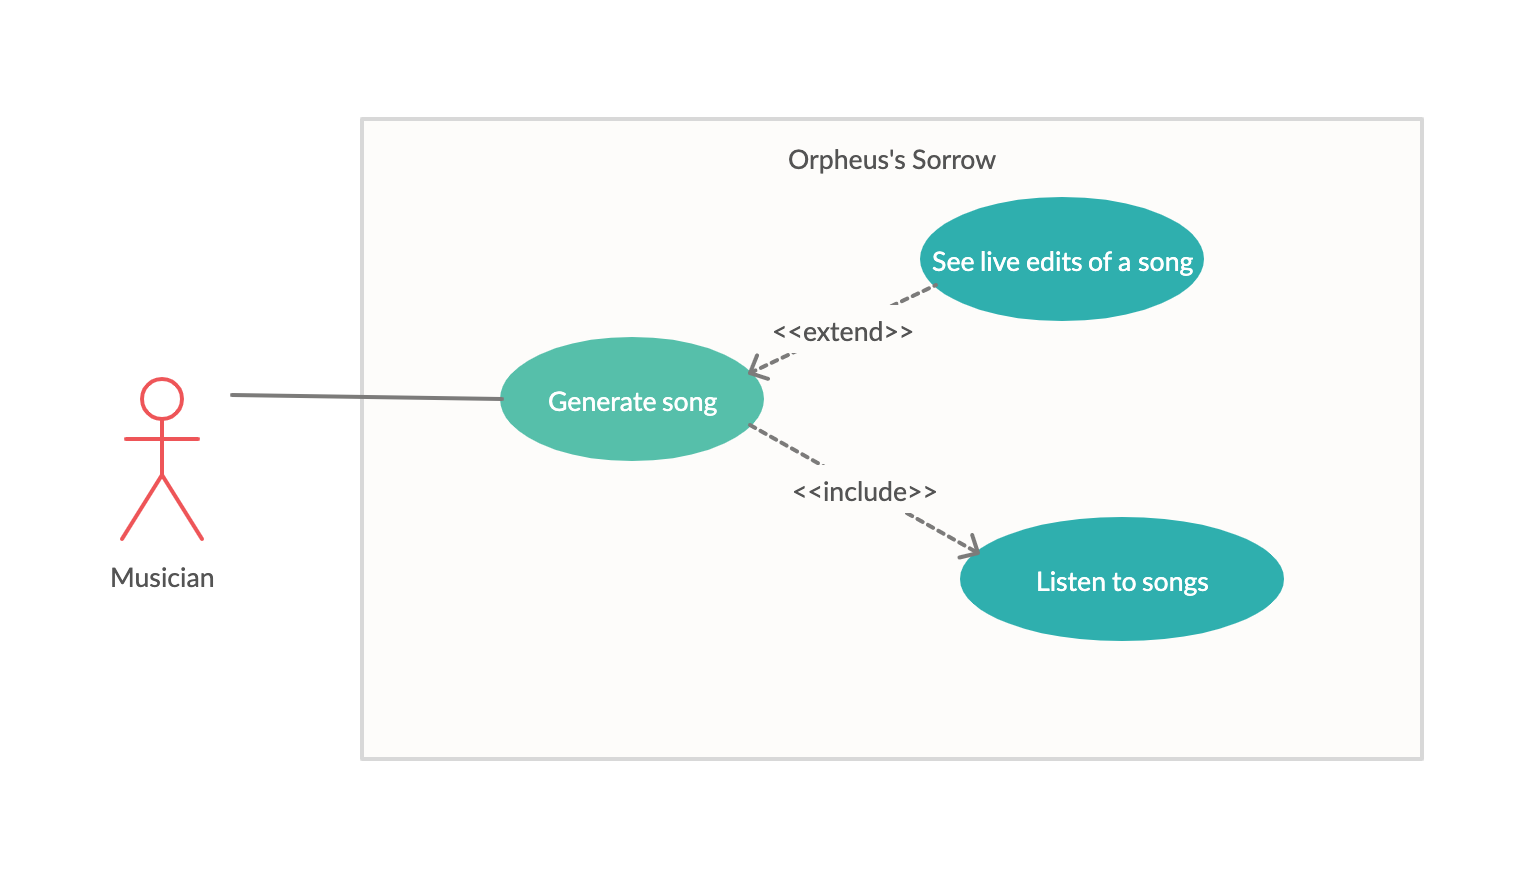
\includegraphics[width=.8\textwidth]{usecase}
  \caption{\emph{UML use case diagram for the main features}}
  \label{fig:usecase}
\end{figure}



\section{Design and implementation}

The application is composed out of two servers,
a React server for the frontend,
and a Flask server for the backend,
as shown in Figure \emph{\ref{fig:application}}.

\begin{figure}[H]
  \centering
  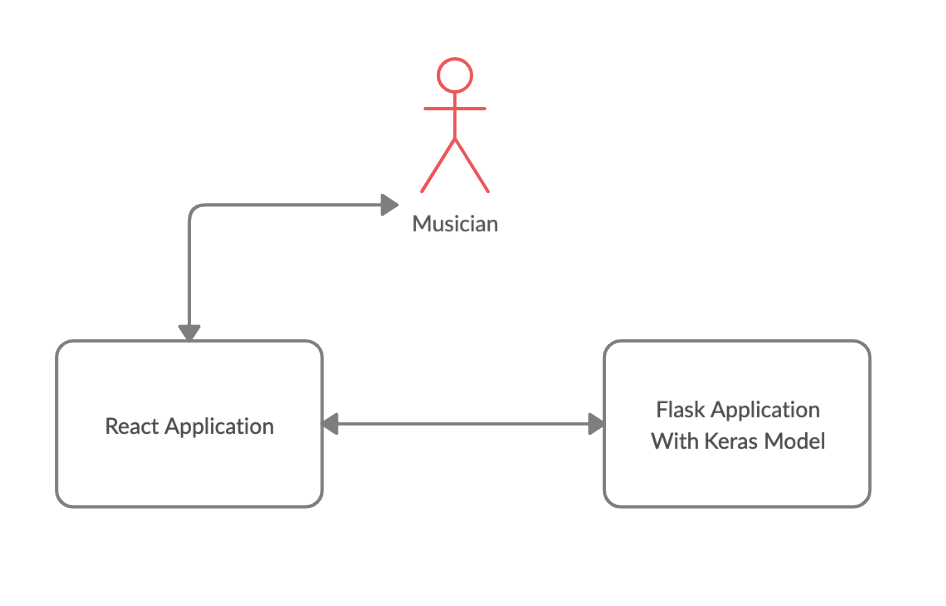
\includegraphics[width=.5\textwidth]{application}
  \caption{\emph{Main structure of the application}}
  \label{fig:application}
\end{figure}


The main aspects of the servers' design and the
interaction between the two of them or between them and
the user are visible in the sequence diagram displayed in Figure 3.
It explains how the application should react to user input,
how the data should be processed and transmitted through the servers,
considering our use cases.
The following paragraphs will present the objects composing the
diagram and the relationships between them.

\begin{figure}[H]
  \centering
  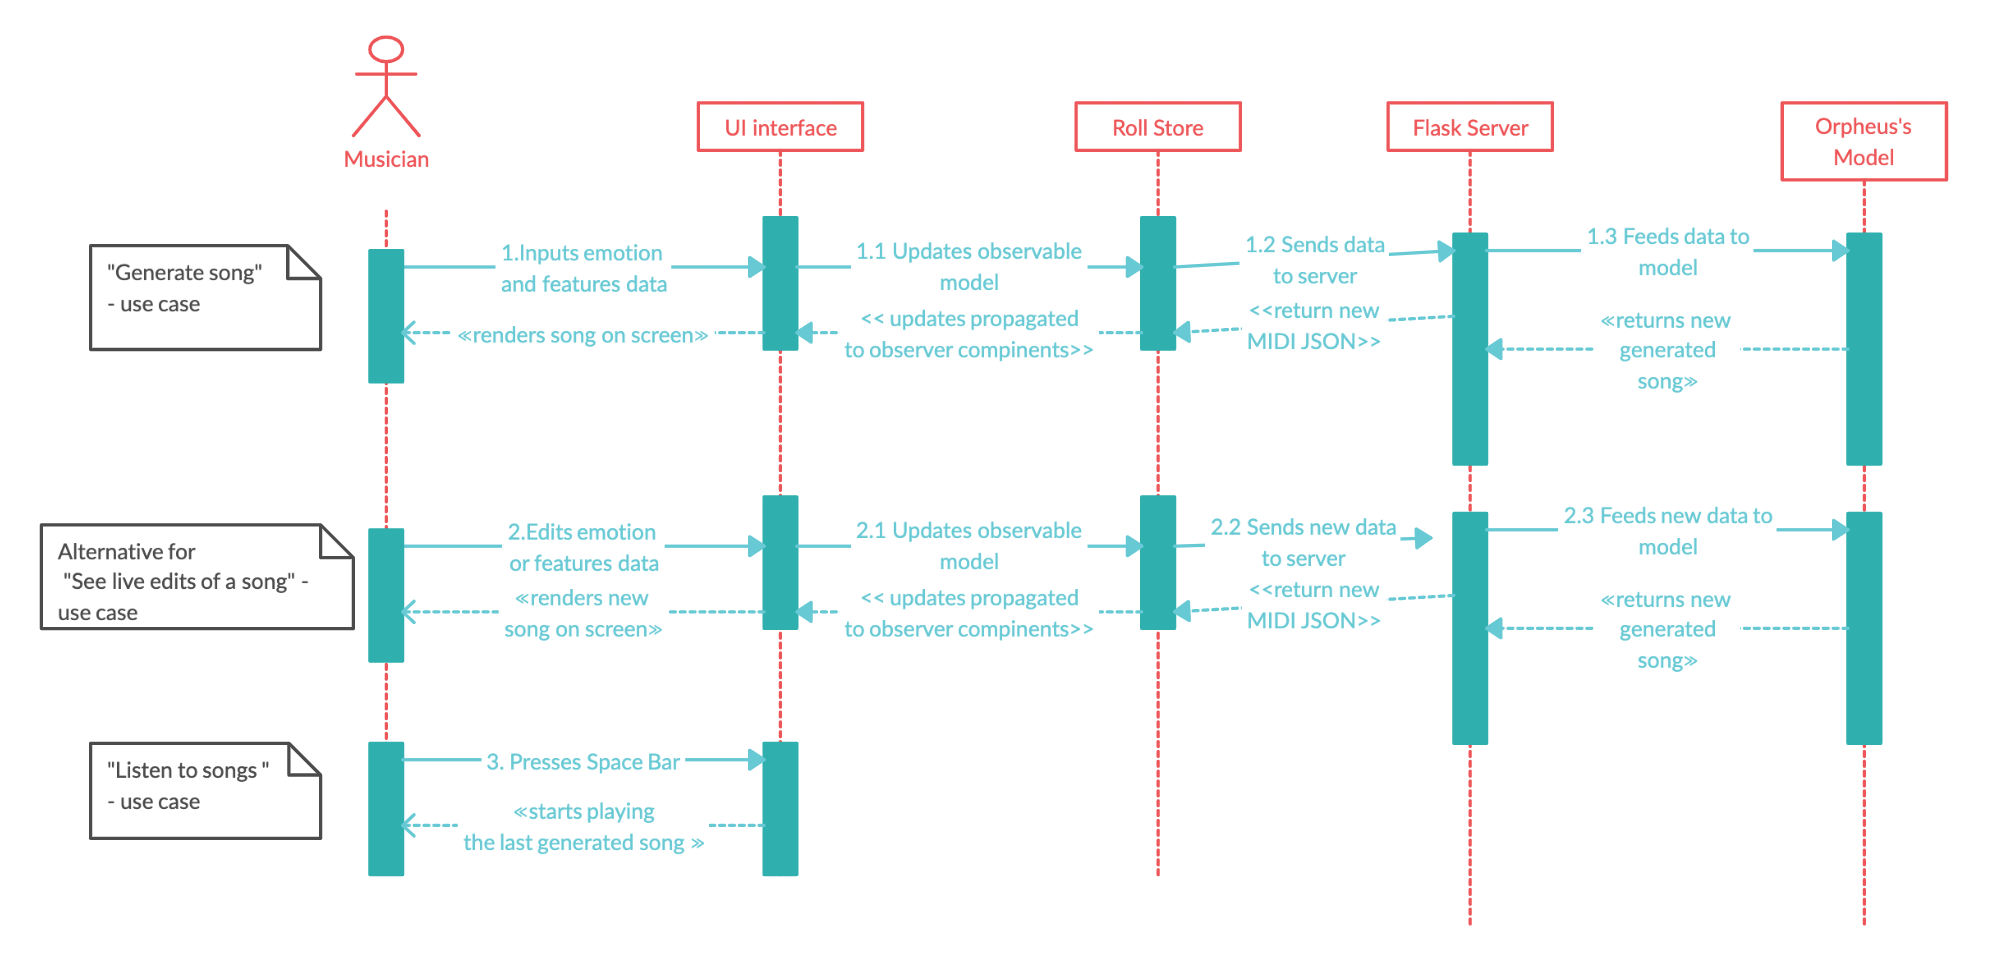
\includegraphics[width=1\textwidth]{sequence}
  \caption{\emph{UML sequence diagram containing the main use cases}}
  \label{fig:sequence}
\end{figure}


\begin{listing}
  \begin{minted}{jsx}
   // Main smart component of our application in which the store is injected
   const MidiContainer = () => {
     const { rollStore } = useStore();
     // other variables
     const memoisedSong = useMemo(() => {
       // mapping request data to our MIDI format
       const songRawBeats = rollStore.pianoRollsSnapshot.map(([roll, x, y]) => [
         roll * 96 + x,
         y + 16
       ]);
       // creating empty beats
       const songBeats = Array.from(Array((16 * 96) / 8), () => [
         [],
         [[INSTRUMENT, [], 1 / 16]]
       ]);
       // adding notes to corresponding beats
       songRawBeats.forEach(([beat, pitch]) => {
         try {
           songBeats[(beat / 8).toFixed(0)][1][0][1] = [
             ...songBeats[(beat / 8).toFixed(0)][1][0][1],
             pitch
           ];
         } catch {/* other error logic */}
       });
       return songBeats;
     }, [rollStore.pianoRollsSnapshot]);
     // Watching for `isPlaying` prop so we start playing the beat accordingly
     useEffect(() => {
       if (isPlaying) { // logic for starting the MIDI player }
       else { // logic for stopping the MIDI player }
     }, [isPlaying, memoisedSong, rollStore.volume]);
    // ... here we add other logic for our components
     return (
       <Wrapper>
         <PlayerContainer
           rolls={rollStore.pianoRollsSnapshot}
           beatIndex={midiRef.current?.beatIndex}
           ... injecting other props here
         />
        {/* other containers */}
       </Wrapper>
     );
   };
  \end{minted}
  \caption{\emph{Example of a smart component}}
  \label{lst:smart}
\end{listing}


The UI interface represents the layer the end-user,
the musician, should interact within all of the use cases.
It is build using the React library,
being composed out of function components and hooks due
to their ease of managing logic,
ease of sharing code between components, and readability.

The interface was designed using the concept of smart and presentational
components \cite{smart_dumb}. The first type refers to components that
should only be concerned about how things look (presentational)
and how to render the data they receive, as seen in Listing \emph{\ref{lst:dumb}};
they should not have any logic regarding the functionalities and
only receive callbacks. The second type defines components
that are concerned about how things work:
they provide data and behavior that is passed down
to presentational components and are linked to state management
libraries, as seen in Listing \emph{\ref{lst:smart}}.

\begin{listing}
  \begin{minted}{jsx}
/**
* Presentational component that renders all keys and positions them
* @param {number} scrollLeft -> value of the scrollLeft position
                                of the Container
*                            -> used for dynamically changing the position of
                                the keys onScroll
*/
const Keys = ({ scrollLeft }) => {
  return (
    <KeysWrapper scrollLeft={scrollLeft}>
      {NOTE_RANGE.map(item => (
        <Key key={item} isSharp={item.indexOf("#") > -1} />
      ))}
    </KeysWrapper>
  );
};
  \end{minted}
  \caption{\emph{Example of presentational component}}
  \label{lst:dumb}
\end{listing}


The Roll Store is our main state management container,
being a MobX-state-tree model,
customized for the application needs,
using the Apisauce wrapper over Axios,
a promise-based HTTP client.
It defines the structure of our data through the Mobx-based
models and the behavior/business logic through Mobx-based actions. It provides the observable data that is injected in the smart components, which, when updated, it triggers re-rendering, such that MobX alongside with React's reconciliation algorithms, reassures the minimum number of components that should update.


The Flask server is a small REST server that is mainly used
as the middleware between the client application and the
Keras model. It exposes a single REST API call,
\emph{generate\_song}, that expects to receive the
input parameters of our application;
an example of the request is the Listing 4
each parameter being explained in the following:
\begin{itemize}
  \item \emph{threshold}, the amount above the value of a generated note should be to be considered valid;
  \item \emph{valence and arousal}, the emotion data;
  \item \emph{features}, the set of the rest of 48 features that can be tweaked in our model;
  \item \emph{multiplier}, the variable used for accentuating the emotion data
\end{itemize}

Orpheus's Model represents the helper class used for creating,
training, evaluating, and loading the Keras model.
It also creates separated models for the encoder and decoder parts
for later use, when generating a new song or
normalizing and creating our metadata.

\begin{listing}[h]
  \centering
  \begin{minted}{js}
{
   "features":[
      45, 
      // ...other features, in total 48
      50
   ],
   "threshold":50,
   "valence":30,
   "arousal":29,
   "multiplier":30
}
  \end{minted}
  \caption{\emph{Example of \textbf{{get\_song}} request}}
  \label{lst:dumb}
\end{listing}

\section{User interface}

This section presents the steps for installing and running the Orpheus's Sorrow
web application on a local machine.
Then it will be discussed the interface of the app alongside the main features.

\subsection{Installation instructions}

Before downloading the application's dependencies,
some prerequisites must be installed and configured on the local machine:
\begin{itemize}
  \item \code{node}, a version above 10.x.x
  \item \code{yarn}, a version above 1.19.x, or \code{npm} above 6.x.x
  \item \code{python}, a version above 3.x with the minimum compatible \code{virtualenv}
\end{itemize}

After the mentioned requirements are satisfied,
one can download the dependencies of the projects.
For the server, one can create a virtual environment in the project's root,
using the command \code{python3 -m venv env}, \code{cd model},
and then install all the project dependencies using
the command \code{python3 -m pip install requirements.txt}.
For the client, one should open a terminal in the project's root,
\code{cd client}, run \code{yarn} (or \code{npm install}),
and wait until all the dependencies are fetched.

To run the full application,
one must run the backend first,
meaning opening a terminal in the project root, \code{cd model},
\code{python3 server.py}.
After that, the frontend can be run by also opening a terminal in the project's root,
\code{cd client}, \code{yarn start} (or \code{npm start})

\subsection{Orpheus's Sorrow interface}

The main UI of the paper's project can be seen in Figure \emph{\ref{fig:interface}}.
It is composed of two parts: the player container (the upper part),
and the input container (the bottom part).
Next, it will be discussed about each container separately.

\begin{figure}[h]
  \centering
  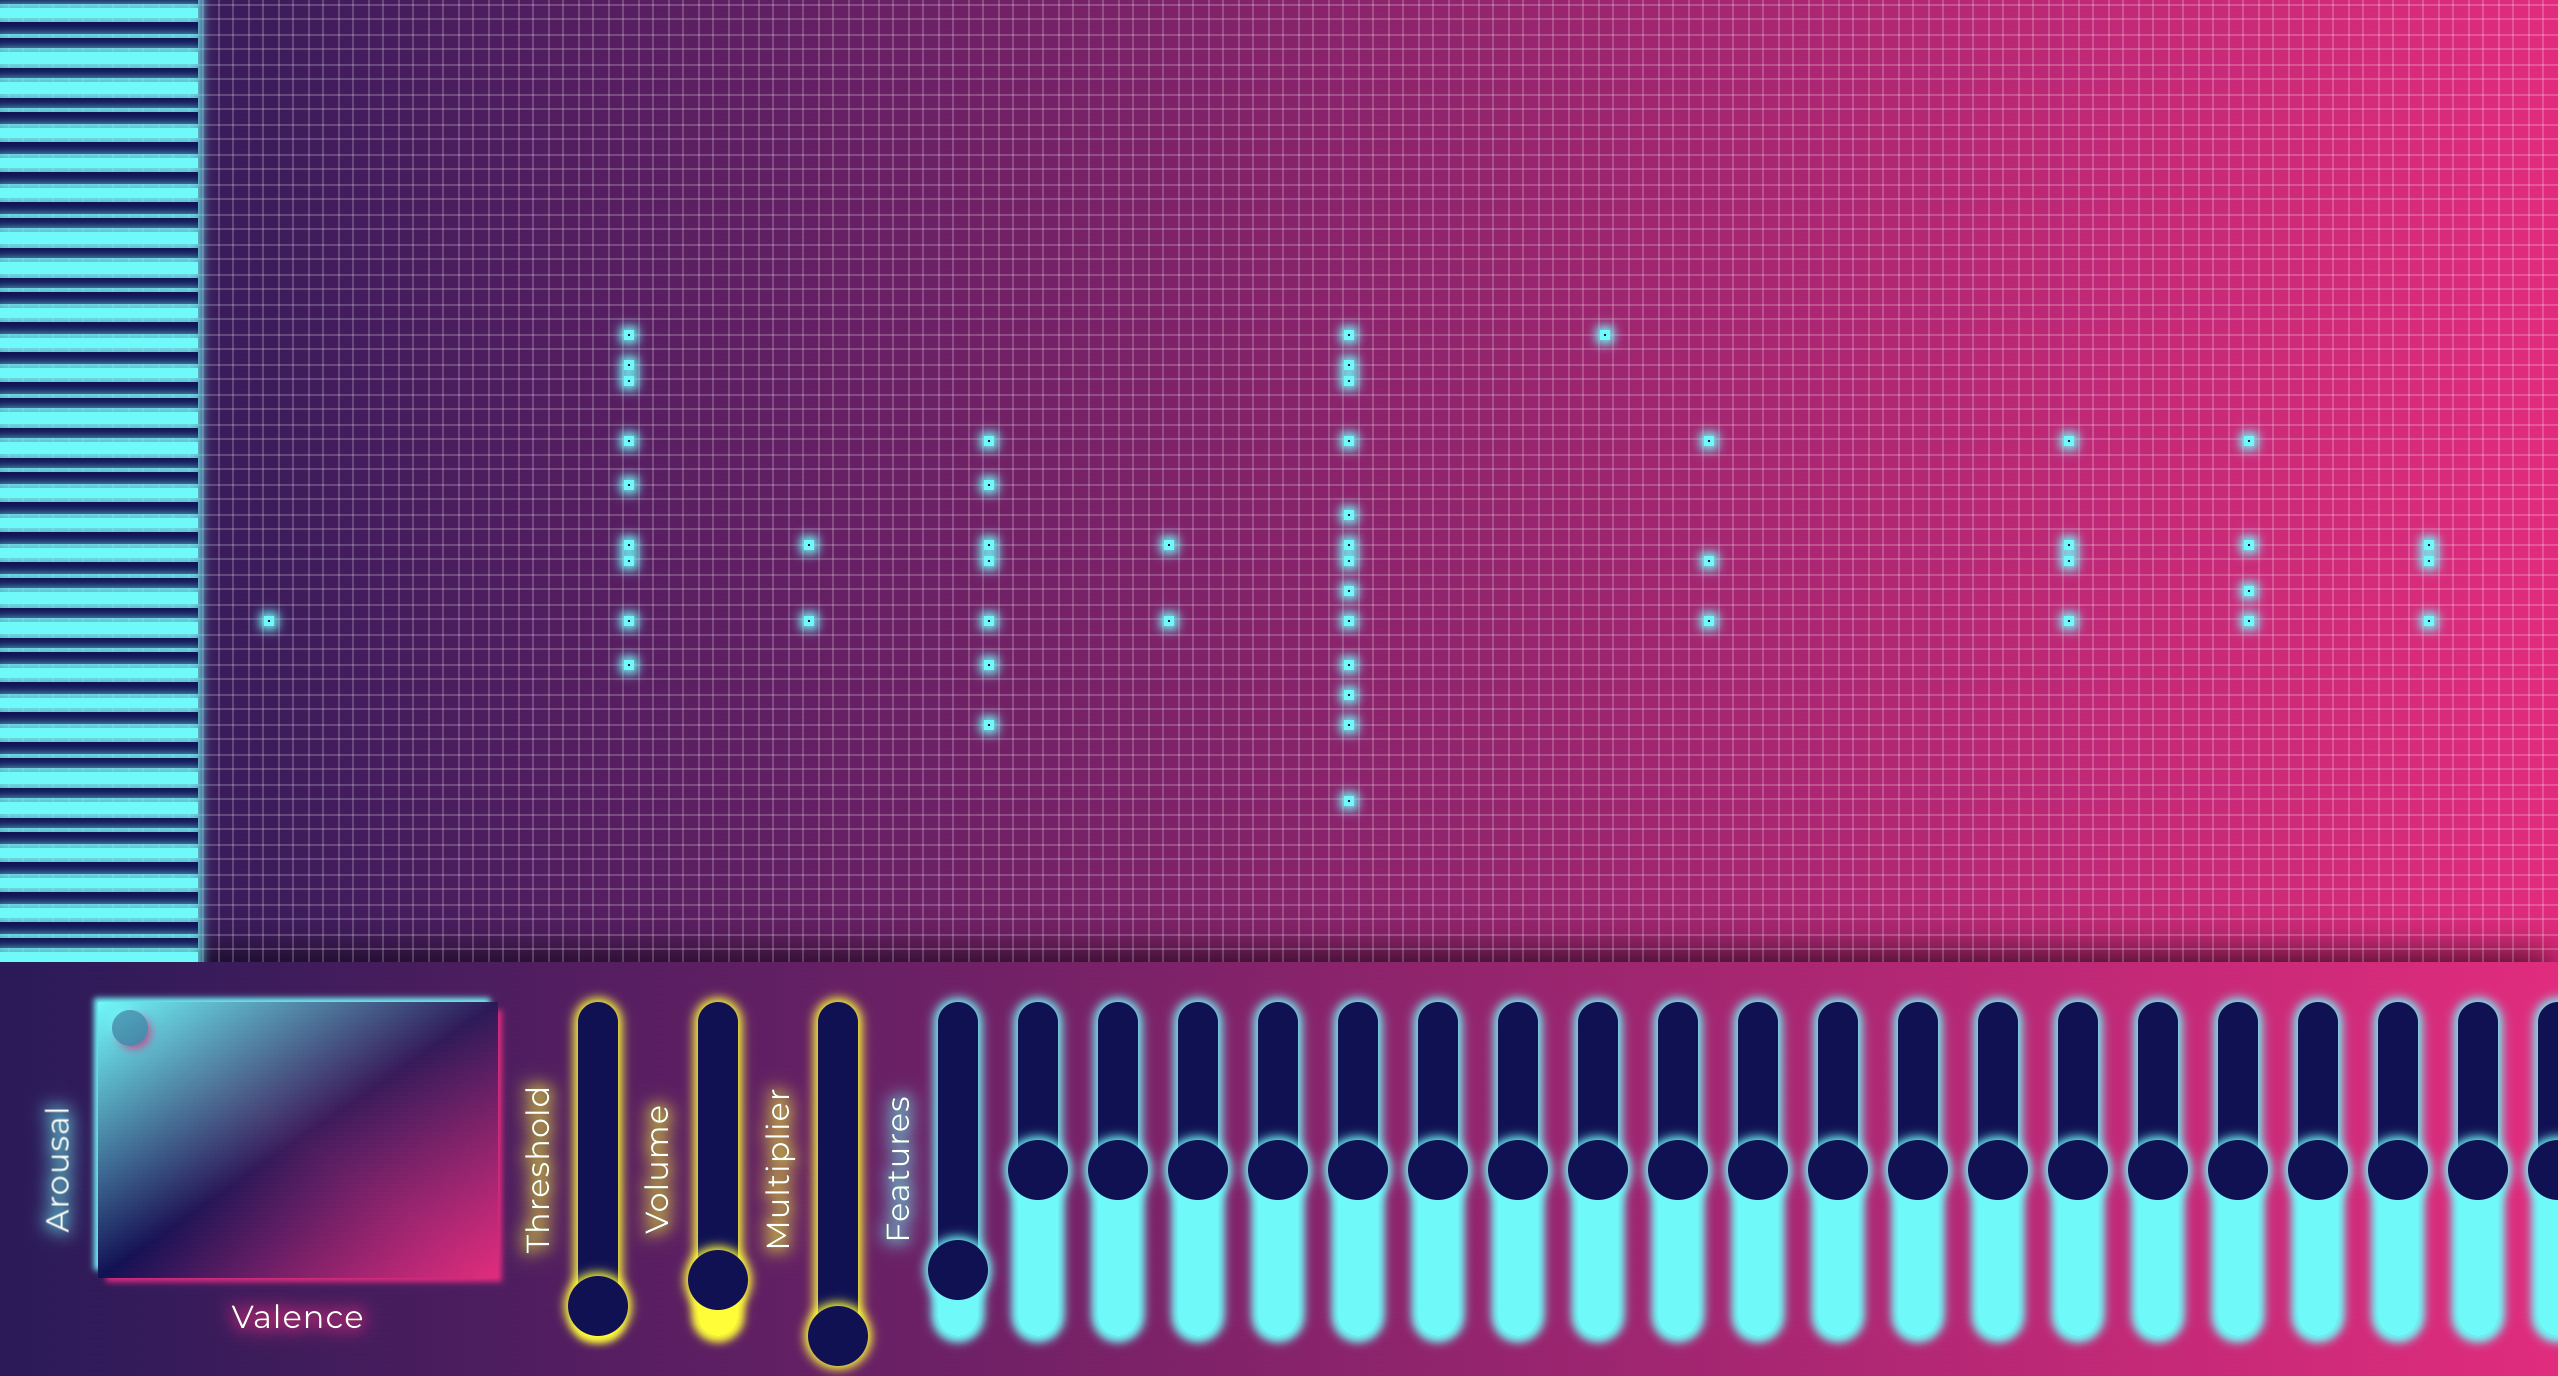
\includegraphics[width=1\textwidth]{interface}
  \caption{\emph{Orpheus's Sorrow interface}}
  \label{fig:interface}
\end{figure}


The first one, the input container,
consists of three main parts: the keys, the notes, and the grid.
The keys position matches the horizontal scroll due to the listener
on the parent container.
The notes and the grid are displayed as a piano roll,
each note being positioned at its location in time and pitch,
the main focus of the grid being to improve readability.
When pressing the spacebar,
the generated song starts playing alongside with the animation of the notes.
They are translated from right to left,
creating the illusion of the notes falling onto the keys and producing
the sound.

The second one, the bottom container,
also consists of three main parts: the emotion input, the meta-inputs,
and the feature inputs.
The emotion input is a 2d/cartesian slider with the x-axis
representing the valence value and the y-axis the arousal value.
The meta-inputs are the threshold, volume, and multiplier sliders.
The first mentioned, as discussed before,
represents the minimum value a note can have to be considered valid.
The volume slider represents the volume of the MIDI player.
When generating songs,
one could desire to amplify the values of the emotion data so the model will be more
influenced by them when composing.
Prompted by this need, the multiplier slider was introduced;
its primary purpose is to be multiplied with the valence and arousal values.
The last part contains the feature sliders that can tweak the other
variables of the features the model identified; in other words,
it changes the structure of the song that is being composed.
When modifying any of the sliders mentioned above, the song is being recomposed,
hence, the possibility to edit the song almost instantaneously,
easing the entire process, which is the principal purpose of the client app.

\chapter{Conclusion and future work}

This paper tries to solve a problem that the aspiring musician has always been fighting,
the music equivalent of "writer's block".
It provides a tool whose primary purpose is to enhance its creational
workflow by taking one of the most challenging tasks off his hands.
Orpheus's Sorrow application offers an easy way of composing songs based on a given feeling,
without the need for mastering music theory.

This trial represents only a proof of concept;
this paper's work is merely scratching the surface of what musical composition implies,
due to solely the complexity of the process,
but thanks to the results,
it has proved itself worthy of investing more time.

The model is capable of composing new songs with a well-defined structure,
based on the input emotion data and features.
Unfortunately, due to the small dataset the network was trained on,
the actual emotions of the generated songs are not that clear.
Despite that,
general characteristics of a song composed based on the given emotions were
found on the newly created compositions,
meaning that the model was able to capture some information about the emotion data.

For future developments,
one of the main improvements for this approach will be to enhance the dataset
with more songs with normal-distributed emotion data;
in this way, the prediction will be more accurate.
Hence the songs will reflect the emotions better.

Another future improvement can be the ability to compose starting
from an already written song,
being able to enhance or continue that piece of music.
This feature can be developed by using the encoder part of the model to predict the
encoding of the given song, attach the emotion data or tweak the values of the encoding,
and then plug the result in the decoder generating a new song.

The client app can also be improved with other features regarding the MIDI player.
One of those could be the ability to edit the created song,
change the playback instrument, and export the new piece as a MIDI file.


% \chapter{Conclusion}
% \input{chapters/conclusion}

% \appendix
% \chapter{Appendix Title}
% \input{chapters/appendix}

% BIBLIOGRAPHY
\bibliographystyle{plain}
\bibliography{references}


\end{document}

% TODO:
% GET THE MODEL FROM GOOGLE COLABS
% WRITE ABOUT GOOGLE COLABS
% CHECK IF IT IS THE SAME WITH THE MODEL FROM LOCAL
% CHECK ALL FILE PATHS

% AWESOME SONG 
% curl 'http://localhost:5000/generate_song' \
%   -H 'Connection: keep-alive' \
%   -H 'Accept: application/json' \
%   -H 'User-Agent: Mozilla/5.0 (Macintosh; Intel Mac OS X 10_14_5) AppleWebKit/537.36 (KHTML, like Gecko) Chrome/83.0.4103.61 Safari/537.36' \
%   -H 'Content-Type: application/json' \
%   -H 'Origin: http://localhost:3000' \
%   -H 'Sec-Fetch-Site: same-site' \
%   -H 'Sec-Fetch-Mode: cors' \
%   -H 'Sec-Fetch-Dest: empty' \
%   -H 'Referer: http://localhost:3000/' \
%   -H 'Accept-Language: en-US,en;q=0.9,ro;q=0.8,co;q=0.7' \
%   --data-binary '{"features":[3,52,93,54,52,50,50,50,50,50,50,50,50,50,50,50,50,50,50,50,50,50,50,50,50,50,50,50,50,50,50,50,50,50,50,50,50,50,50,50,50,50,50,50,50,50,50,50],"threshold":8,"valence":85,"arousal":13,"multiplier":3}' \
%   --compressed

% curl 'http://localhost:5000/generate_song' \
%   -H 'Connection: keep-alive' \
%   -H 'Accept: application/json' \
%   -H 'User-Agent: Mozilla/5.0 (Macintosh; Intel Mac OS X 10_14_5) AppleWebKit/537.36 (KHTML, like Gecko) Chrome/83.0.4103.61 Safari/537.36' \
%   -H 'Content-Type: application/json' \
%   -H 'Origin: http://localhost:3000' \
%   -H 'Sec-Fetch-Site: same-site' \
%   -H 'Sec-Fetch-Mode: cors' \
%   -H 'Sec-Fetch-Dest: empty' \
%   -H 'Referer: http://localhost:3000/' \
%   -H 'Accept-Language: en-US,en;q=0.9,ro;q=0.8,co;q=0.7' \
%   --data-binary '{"features":[50,50,50,50,50,50,50,50,50,50,50,50,50,50,50,50,50,50,50,50,50,50,50,50,50,50,50,50,50,50,50,50,50,50,50,50,50,50,50,50,50,50,50,50,50,50,50,50],"threshold":8,"valence":86,"arousal":75,"multiplier":3}' \
%   --compressed

% curl 'http://localhost:5000/generate_song' \
%   -H 'Connection: keep-alive' \
%   -H 'Accept: application/json' \
%   -H 'User-Agent: Mozilla/5.0 (Macintosh; Intel Mac OS X 10_14_5) AppleWebKit/537.36 (KHTML, like Gecko) Chrome/83.0.4103.61 Safari/537.36' \
%   -H 'Content-Type: application/json' \
%   -H 'Origin: http://localhost:3000' \
%   -H 'Sec-Fetch-Site: same-site' \
%   -H 'Sec-Fetch-Mode: cors' \
%   -H 'Sec-Fetch-Dest: empty' \
%   -H 'Referer: http://localhost:3000/' \
%   -H 'Accept-Language: en-US,en;q=0.9,ro;q=0.8,co;q=0.7' \
%   --data-binary '{"features":[100,57,15,72,44,50,50,50,50,50,50,50,50,50,50,50,50,50,50,50,50,50,50,50,50,50,50,50,50,50,50,50,50,50,50,50,50,50,50,50,50,50,50,50,50,50,50,50],"threshold":10,"valence":16,"arousal":24,"multiplier":2}' \
%   --compressed

% curl 'http://localhost:5000/generate_song' \
%   -H 'Connection: keep-alive' \
%   -H 'Accept: application/json' \
%   -H 'User-Agent: Mozilla/5.0 (Macintosh; Intel Mac OS X 10_14_5) AppleWebKit/537.36 (KHTML, like Gecko) Chrome/83.0.4103.61 Safari/537.36' \
%   -H 'Content-Type: application/json' \
%   -H 'Origin: http://localhost:3000' \
%   -H 'Sec-Fetch-Site: same-site' \
%   -H 'Sec-Fetch-Mode: cors' \
%   -H 'Sec-Fetch-Dest: empty' \
%   -H 'Referer: http://localhost:3000/' \
%   -H 'Accept-Language: en-US,en;q=0.9,ro;q=0.8,co;q=0.7' \
%   --data-binary '{"features":[100,57,15,72,44,50,50,50,50,50,50,50,50,50,50,50,50,50,50,50,50,50,50,50,50,50,50,50,50,50,50,50,50,50,50,50,50,50,50,50,50,50,50,50,50,50,50,50],"threshold":10,"valence":16,"arousal":24,"multiplier":2}' \
%   --compressed